\section{Evaluation}
% \begin{figure*}[t!]
    \centering
    \begin{subfigure}[t]{0.45\textwidth}
        \includegraphics[width=0.9\textwidth]{images/black_box_radar.png}
        \caption{Performance of the black-box models.}
        \label{fig:first}
    \end{subfigure}
    \begin{subfigure}[t]{0.45\textwidth}
        \includegraphics[width=0.9\textwidth]{images/white_box_radar.png}
        \caption{Performance of the open-source models.}
        \label{fig:second}
    \end{subfigure}
    \caption{Overall performance of nine models on a snapshot within 4k context length of Minerva.}
    \label{fig:radar}

\end{figure*}

\subsection{Experimental Setup}
We use the proposed framework to evaluate nine widely used language models on a fixed snapshot of 1110 randomly generated test samples. For all tests, we fixed the context length to 4k tokens, except in the Stateful Processing category, where the context length depends on the number of operation steps. We set the number of steps as 200 for quantity state and 100 for set state, corresponding to an approximate context length of 1.5k tokens. For evaluation, we use exact match accuracy for binary tasks, ROUGE-L\citep{lin-2004-rouge} for tests that require sequence overlap measurement, and Jaccard similarity \citep{jaccard1901etude} for set overlap. Further details on the number of examples, hyperparameter configurations, and evaluation metrics for the tests are provided in Appendices \ref{apd:task_detail} and \ref{apd:eval}.

The evaluated models are divided into two groups: 

\textbf{Black-box models}: GPT-4-turbo, GPT-4o, GPT-4o-mini, and Cohere-command-rplus. 

\textbf{Open-source models}: Mistral-7b-instruct-v02, Phi-3-small-128k-instruct (7B), LLaMA-3.1-8b-instruct, Gemma-2-9b, and Phi-3-medium-128k-instruct (14B).

We set the max output token to 4096, temperature to 0, and top\_p to 1 for all model inference.



\subsection{Model Performance Overview}

Figure \ref {fig:radar} summarizes the overall performance of the evaluated models on the memory test snapshot within 4k context length. Notably, this context length is usually considered short for context utilization benchmarks, and many models are expected to perform perfectly at this length. However, our evaluation reveals significant disparities in performance across the capabilities, even within this manageable context length. Overall, the GPT-4-turbo/GPT-4o models show stronger all-around performance across the capabilities. In contrast, other models excel at the search task but struggle significantly in other areas, leading to a widening performance gap compared to stronger models. This is especially evident in the \textbf{Stateful Processing} tasks, where models exhibit steep performance drops. Even within the GPT-4(o) models, there were noticeable variations in performance across different tasks, despite them being the best-performing models. This suggests that strong performance in simple retrieval tasks does not imply effective context processing, highlighting that using NIAH-like tests alone for evaluating context utilization is not sufficient to capture the full spectrum of model capabilities. Our framework instead reveals significant variability in performance across distinct capability categories, offering a more nuanced understanding of model limitations.

The following sections analyze each test type in detail, highlighting key insights from the evaluations.


\subsection{Analysis on Atomic Tests}


\section{Structure Search with Program Synthesis}\label{sec:algo}
%
\subsection{Preliminaries}
\begin{definition}[Tensor, Tensor Size]
Let $d \in \nat$ and $n_1, n_2, \ldots, n_d \in \nat$.
%
A tensor $\ten{T} \in \real^{n_1 \times n_2 \times \cdots \times n_d}$ is a $d$-dimensional array.
%
Each dimension $\mu \in \{1, 2, \ldots, d\}$ has a name $I_\mu$ and $\size{I_\mu} = n_\mu$.
%
We use $\ten{T}_{i_1, i_2, \ldots, i_d}$ to denote an element in the tensor where $i_\mu \in \{1, \ldots, n_\mu\}$.
%
The size of the tensor $\ten{T}$ is defined as $\size{\ten{T}} = \prod_{\mu=1}^{d} n_\mu$.
\end{definition}

\begin{definition}[Matricization]
For a $d$-dimensional tensor $\ten{T} \in \real^{n_1 \times n_2 \times \cdots \times n_d}$ and a set of dimensions $\ind_s \subseteq \{I_1,\ldots, I_d\}$, let $\ind_t = \{I_1, \ldots, I_d\}\ \backslash\ \ind_s$ be the complementary mode set, $\ten{T}' = \mathtt{permute}\left(\ten{T}, [\mu]_{I_\mu \in \ind_s} + [\nu]_{I_\nu \in \ind_t}\right)$ be the permuted tensor with the modes $s$ at the front, then the corresponding \emph{$\ind_s$-matricization} $\matric{T}{\ind_s}$ is defined as $
\matric{T}{\ind_s} = \mathtt{reshape}\left(\ten{T}', \prod_{I_\mu \in \ind_s} n_{\mu}, \prod_{I_\nu \in \ind_t} n_{\nu}\right)$.
\end{definition}
\begin{definition}[Tensor Network]
A tensor network is an undirected graph $G=(\nodes,\edges)$ where each vertex in $\nodes$ is a tensor and each edge in $\edges$ is a tuple of three elements: two node names and their shared index name. Particularly, tensor networks without cycles are called \emph{tree tensor networks}. The tensor represented by a graph $G$ is the contraction of all tensors over shared modes, denoted by $\net{G}$. The size of a tensor network is $\size{G} = \sum_{\ten{T} \in \nodes} \size{\ten{T}}$.
\end{definition}
%
Given a tensor network $G$, we call edges with a dangling end \emph{free edges}, and those without dangling ends \emph{contracted edges}.
%
For example, the network in \autoref{fig:example-program} has four free edges $I_1, I_2, I_3, I_4$ and three contracted edges $r_1, r_2, r_3$.
%
The tensor represented by this network is computed as
$
\net{G}_{ijkl} = \sum_{a=1}^{r_1}\sum_{b=1}^{r_2}\sum_{c=1}^{r_3} \ten{A}_{ia}\ten{B}_{jb}\ten{C}_{abc}\ten{D}_{c k l}
$

\begin{definition}[Tensor Network Structure Search]
The tensor network structure search (TN-SS) problem finds the optimal tensor network that reduces the storage space while maintaining accuracy. Specifically, given a TN-SS problem $(\ten{T}, \error)$ where $\ten{T}$ is the data tensor and $\error$ is a prescribed error bound, the goal of the TN-SS algorithm is to solve the following optimization problem
$$
\arg\min_{G} \quad \size{G} \quad
\textrm{s.t.} \quad \norm{\net{G} - \ten{T}}\leq \error\norm{\ten{T}}
$$
\end{definition}
In other words, the TN-SS problem aims at finding the most compressed tensor network within a given error bound.
%
In this work, we target arbitrary tree structures and do not consider structures with cycles.

\begin{algorithm}[t]
\small
\captionsetup{font=small} % set size of caption font
\caption{Tensor network structure search algorithm}\label{alg:high-level}
\begin{algorithmic}[1]
    \Require The data tensor $\ten{T}$, the error bound $\error$, the param $k$
    \Ensure The result tensor network $G$ such that $\size{G} \leq \size{\ten{T}}$, and $\norm{\net{G} - \ten{T}} \leq \error \norm{\ten{T}}$
    \Function{SearchStructure}{$\ten{T}, \error, k$}
        \State $G_0 \gets (\{\ten{T}\}, \emptyset)$
        \State $G_{min} \gets G_0$
        \For{$(G, \error') \in \textsc{Synth}(\ten{T}, \error, k)$}
            \State $G \gets$ \Call{Round}{$G, \error'$}
            \If{$\size{G} < \size{G_{min}}$}
                \State $G_{min} \gets G$
            \EndIf
        \EndFor
        \State \Return $G_{min}$
    \EndFunction
\end{algorithmic}
\end{algorithm}

\subsection{From TN-SS To Program Synthesis}\label{sec:algo:program}
%
To solve a TN-SS problem $(\ten{T},\error)$, we propose to find a near-optimal solution by generating a transformation program that incrementally splits nodes to produce a tensor network with reduced size.
%
The algorithm that integrates program synthesis with TN-SS is presented in~\cref{alg:high-level}.
%
The process begins by constructing an initial graph $G_0$ containing a single node $\ten{T}$.
%
Then, the algorithm enters a loop, where it repeatedly calls the function \textsc{Synth} (Line 4).
%
This function uses a program synthesizer to enumerate and execute transformation programs, generating various tensor networks $G$.
%
At the end of each iteration, the algorithm calls the procedure \textsc{Round} for further compression, and updates the current minimum structure $G_{min}$ if the newly generated structure has a lower cost.
%
Finally, the algorithm returns the structure with the minimum cost.
%
In the remaining section, we introduce the design of the transformation language and the formal reduction of TN-SS to program synthesis.

\begin{figure}[t]
    \centering
    \small
    \vspace{-1em}
    \begin{alignat*}{2}
        \text{Programs or sketches}\quad & P,\sketch && := \emptyprog \mid \expr \mid \seq{P}{\expr} \\
        \text{Expressions}\quad & \expr &&:= \osplit(\ind, r) \\
        \text{Index sets}\quad & \ind  &&:= \{I_\mu\} \mid \ind \cup \{I_\mu\} \\
        \text{Ranks or holes}\quad & r     &&:=\ \hole \mid 1 \mid 2 \mid \cdots \\
        \text{Dimensions}\quad & \mu   &&:= 1, 2, 3, \ldots
    \end{alignat*}
    \vspace{-2em}
    \begin{align*}
    \sem{E}(\bot) = \bot \quad&\quad \sem{\emptyprog}(G, \error) = (G, \error) \\
    \sem{\osplit(\indices, r)}(G, \error) &= \textsc{ExecOSplit}(G, \error, \ind, r)\\
    \sem{\seq{P}{\expr}}(G,\error) &= \sem{\expr}(\sem{P}(G,\error))
    \end{align*}
    \vspace{-2em}
    \caption{Syntax and semantics for the DSL.}\label{fig:dsl}
    % \vspace{-1em}
\end{figure}

\paragraph{Syntax and Semantics of the Language}
%
As illustrated in~\cref{fig:dsl}, a program $P$ can either be empty, denoted by $\emptyprog$, or a sequence of expressions $\seq{P}{E}$.
%
Each expression represents a split operation that takes a set of indices $\ind$ and a rank $r$ as inputs.
%
The index set consists of indices from different modes $I_\mu$.
%
The rank $r$ can be either an integer or a hole $\hole$, which can be filled later.
%
If a program consists of ranks as holes, it is referred to as a \emph{program sketch}.
%
A sketch $\sketch$ can be completed with a rank assignment $\many{\hole_s \mapsto r_s}$ (we use $\many{X}$ to denote a set of similar elements), which is a mapping from holes to integers.
%
A rank assignment can \emph{complete} a sketch by filling holes with corresponding integers, resulting in a complete program, represented as $\sketch[\many{\subst{\hole_s}{r_s}}]$.
%
The execution of a complete program $\sem{P}$ takes a tensor network $G$ and an error bound $\error$ as inputs, and outputs a new tensor network $G'$ and the remaining error bound $\error' \leq \error$.
%
If an execution fails, it skips the remaining expressions and return $\bot$.
%
Multiple expressions in a program are executed sequentially.
%
For each split operation, it is executed using the method \textsc{ExecOSplit}, which produces an updated tensor network while ensuring the result stays within the specified error bound.
%
For example, \cref{fig:example-program} (left) shows a program of three splits.
%
Its execution produces the network structure depicted on the right.
%
The steps of how this result is reached is detailed in \cref{fig:output-directed-example}, and further explained in \cref{sec:algo:split}.

\paragraph{Reduction to Program Synthesis}
%
Using the language defined above, we reduce the TN-SS problem $(\ten{T}, \error)$ to an optimal program synthesis problem:
\begin{align*}
\arg\min_{P}~\size{G} \quad
\textrm{s.t.} \quad \sem{P}(G_0, \error) = (G, \error^{*}) \land \error \leq \error^{*}
\end{align*}
where $G_0 = (\{\ten{T}\}, \emptyset)$ is the initial tensor network containing the data tensor and $\error^{*}$ is the remaining error.
%
Its solution is a program, execution of which produces a tensor network $G$ of the smallest size within the error bound $\error$.

\cref{alg:synth} outlines our high-level program synthesis algorithm.
%
The core idea is to enumerate and rank sketches, and then complete sketches by filling in their holes.
%
The algorithm starts from an empty sketch, and incrementally appends new expressions to construct all possible sketches (Line 3-7).
%
The details of sketch construction and the implementation of the function \validexpr\ are described in \cref{sec:algo:split}.
%
Then, the algorithm fills holes in each sketch and creates complete programs that generate various network structures.
%
As the last step, the algorithm extracts the top-$k$ network structures according to their approximated costs (Line 12).
%
Both the sketch completion algorithm and the cost computation are elaborated in \cref{sec:algo:fillhole}.

\begin{algorithm}[t]
\small
\captionsetup{font=small} % set size of caption font
\caption{The high-level program synthesis algorithm}\label{alg:synth}
\begin{algorithmic}[1]
    % \Require The data tensor $\ten{T}$, the error bound $\error$, the param $k$
    % \Ensure Networks $Gs$ such that $\norm{\net{G}-\ten{T}} \leq \error \norm{\ten{T}}$
    \Function{Synth}{$\ten{T}, \error, k$}
        \State $\sketch s, Gs \gets \{\emptyprog\}, \emptyset$
        \For{$\sketch \in Ss$} %\Comment{Compute all sketch structures}
            \For{$\expr \in \validexpr(\ten{T}, \sketch)$}
                \For{$P \in \fillholes(\seq{\sketch}{\expr}, \error)$}
                    \State $(G, \error') \gets \sem{P}(G_0, \error)$
                    \State $Gs \gets Gs \cup \{(G, \error')\}$
                \EndFor
                \State $Ss \gets Ss \cup \{\seq{\sketch}{\expr}\}$
            \EndFor
        \EndFor
        \State \Return{\Call{TopK}{$Gs, k$}}
    \EndFunction
\end{algorithmic}
\end{algorithm}

\subsection{Programs with Output-Directed Splits}\label{sec:algo:split}
%
\paragraph{Output-Directed Splits}
%
An output-directed split expression $\osplit(\ind, r)$ takes two arguments: a partition block $\ind$ of free indices from the data tensor and a target rank $r$.
%
The semantic of this expression is as follows: given a tensor network $G$ and an error bound $\error$, the expression transforms $G$ by splitting a node into two.
%
The resulting edge connecting the two new nodes forms a free index partition that includes the block $\ind$.
%
\cref{fig:output-directed-example} provides a step-by-step walk-through of the execution of output-directed splits from the program shown in \cref{fig:example-program}.
%
In step \textcircled{\scriptsize 1}, the split expression aims to create a partition where one block is $\{I_1\}$.
%
Since the current network consists of a single node $\ten{T}$, it is picked and split into $\ten{T}_1$ and $\ten{T}_2$.
%
A new edge labelled $r_1$ is created between them, dividing the free indices into two disjoint sets $\{I_1\}$ and $\{I_2, I_3, I_4\}$ and thereby satisfying the split requirement.
%
In step \textcircled{\scriptsize 2}, the goal is to form a new partition block $\{I_1, I_2\}$.
%
The execution procedure discovers that splitting $\ten{T}_2$ and isolating $I_2$ and $r_1$ fulfills the requirement.
%
Finally, step \textcircled{\scriptsize 3} expects to further split a previously created partition block.
%
Splitting the node $\ten{T}_3$ at the index $I_2$ meets the expectation.

The key idea of executing output-directed splits is to convert $\osplit(\ind, r)$ into equivalent, natural node splits $\isplit(\ten{T}, \ind_s, r)$, which takes the node name as arguments and we call them \emph{input-directed splits}.
%
Execution of an input-directed split is built on truncated singular value decomposition (SVD) with minor modifications.
%
Due to the space limitation, we leave the details of output- and input-directed splits to \cref{sec:appendix:alg}.
%
Note that the execution of output-directed splits may fail if the combination  is invalid.
%
For instance, $\osplit(\{I_1, I_2\}, r)$ followed by $\osplit(\{I_1, I_3\}, r)$ is invalid as we cannot put the index $I_1$ in two partition blocks if one is not a subset of the other.
%
%
During program synthesis, the function \validexpr\ in~\cref{alg:synth} takes charge of filtering out invalid combinations to avoid failures.
%

\begin{figure}[t]
    \centering
    \resizebox{0.85\linewidth}{!}{
    \begin{tikzpicture}
\Vertex[x=1,y=1,label=\ten{T},Math,size=.5,color=splitcolor]{G}
\Vertex[x=0,y=1,IdAsLabel,style={color=white},Math,size=.5]{I_1}
\Vertex[x=0.5,y=1.75,IdAsLabel,style={color=white},Math,size=.5]{I_2}
\Vertex[x=1.5,y=1.75,IdAsLabel,style={color=white},Math,size=.5]{I_3}
\Vertex[x=2,y=1,IdAsLabel,style={color=white},Math,size=.5]{I_4}
\Edge(I_1)(G)
\Edge(I_2)(G)
\Edge(I_3)(G)
\Edge(I_4)(G)

\node[circle, draw, minimum size=0.1cm, inner sep=1pt, align=center] (step) at (2.7,1.25) {\tiny 1};
\draw[->] (2.5, 1) node {} -- node[anchor=south]{\scriptsize $\quad\osplit(\{I_1\}, r_1)$} (5, 1) node {};

\Vertex[x=5.5,y=1,label=\ten{T}_1,Math,size=.5,color=splitcolor]{G_1}
\Vertex[x=6.5,y=1,label=\ten{T}_2,Math,size=.5,color=splitcolor]{G_2}
\Vertex[x=5.5,y=2,label=I_1,style={color=white},Math,size=.5]{I1_1}
\Vertex[x=6.5,y=2,label=I_2,style={color=white},Math,size=.5]{I2_1}
\Vertex[x=7.25,y=1.75,label=I_3,style={color=white},Math,size=.5]{I3_1}
\Vertex[x=7.5,y=1,label=I_4,style={color=white},Math,size=.5]{I4_1}
\Edge(I1_1)(G_1)
\Edge(I2_1)(G_2)
\Edge(I3_1)(G_2)
\Edge(I4_1)(G_2)
\Edge[color=splitcolor,lw=2,label=r_1,Math,position=above](G_1)(G_2)
% \draw[dashed,thick,orange] (5,2) node {} -- (5,0) node {};
% \draw[dashed,thick] (4.05,0.5) rectangle (6,1.5);


% \draw[->] (7, 1) node {} -- node[anchor=south]{\scriptsize $\opsplit(\{I_1, I_2\})$} (9, 1) node {};

% \Vertex[x=9.5,y=1,label=G_1,Math]{G1_2}
% \Vertex[x=10.5,y=1,label=G_3,Math]{G3}
% \Vertex[x=11.5,y=1,label=G_4,Math]{G4}
% \Vertex[x=9.5,y=2,label=I_1,style={color=white},Math]{I1_2}
% \Vertex[x=10.5,y=2,label=I_2,style={color=white},Math]{I2_2}
% \Vertex[x=11.5,y=2,label=I_3,style={color=white},Math]{I3_2}
% \Vertex[x=11.5,y=0,label=I_4,style={color=white},Math]{I4_2}
% \Edge(I1_2)(G1_2)
% \Edge(I2_2)(G3)
% \Edge(I3_2)(G4)
% \Edge(I4_2)(G4)
% \Edge[label=r_1,Math,position=above](G1_2)(G3)
% \Edge[color=orange,lw=2,label=r_2,Math,position=above](G3)(G4)
% % \draw[dashed,thick,orange] (11,2) node {} -- (11,0) node {};

% \draw[->] (0, -2) node {} -- node[anchor=south]{\scriptsize $\opsplit(\{I_2\})$} (1.5, -2) node {};

% \Vertex[x=3,y=-1.5,label=G_1,Math]{G1_3}
% \Vertex[x=3,y=-2.5,label=G_5,Math]{G5}
% \Vertex[x=4,y=-2,label=G_6,Math]{G6}
% \Vertex[x=5,y=-2,label=G_4,Math]{G4_3}
% \Vertex[x=2,y=-1,label=I_1,style={color=white},Math]{I1_3}
% \Vertex[x=2,y=-3,label=I_2,style={color=white},Math]{I2_3}
% \Vertex[x=5,y=-1,label=I_3,style={color=white},Math]{I3_3}
% \Vertex[x=6,y=-2,label=I_4,style={color=white},Math]{I4_3}
% \Edge(I1_3)(G1_3)
% \Edge(I2_3)(G5)
% \Edge(I3_3)(G4_3)
% \Edge(I4_3)(G4_3)
% \Edge[label=r_1,Math,position=above right](G1_3)(G6)
% \Edge[color=orange,lw=2,label=r_3,Math,position=below right](G5)(G6)
% \Edge[label=r_2,Math,position=above](G6)(G4_3)
% % \draw[dashed,thick,orange] (3,-2) node {} -- (4,-3) node {};

% \draw[->] (6.5, -2) node {} -- node[anchor=south]{\scriptsize $\opsplit(\{I_4\})$} (8, -2) node {};

% \Vertex[x=9.5,y=-1.5,label=G_1,Math]{G1_4}
% \Vertex[x=9.5,y=-2.5,label=G_5,Math]{G5_4}
% \Vertex[x=10.5,y=-2,label=G_6,Math]{G6_4}
% \Vertex[x=11.5,y=-2,label=G_7,Math]{G7}
% \Vertex[x=12.5,y=-2,label=G_8,Math]{G8}
% \Vertex[x=8.5,y=-1,label=I_1,style={color=white},Math]{I1_4}
% \Vertex[x=8.5,y=-3,label=I_2,style={color=white},Math]{I2_4}
% \Vertex[x=11.5,y=-1,label=I_3,style={color=white},Math]{I3_4}
% \Vertex[x=12.5,y=-1,label=I_4,style={color=white},Math]{I4_4}
% \Edge(I1_4)(G1_4)
% \Edge(I2_4)(G5_4)
% \Edge(I3_4)(G7)
% \Edge(I4_4)(G8)
% \Edge[label=r_1,Math,position=above right](G1_4)(G6_4)
% \Edge[label=r_3,Math,position=below right](G5_4)(G6_4)
% \Edge[label=r_2,Math,position=above](G6_4)(G7)
% \Edge[color=orange,lw=2,label=r_4,Math,position=above](G7)(G8)
% \draw[dashed,thick,orange] (12,-1) node {} -- (12,-3) node {};


\end{tikzpicture}
    }
    \resizebox{0.95\linewidth}{!}{
    \begin{tikzpicture}
\Vertex[x=4.5,y=1,label=\ten{T}_1,Math,size=.5]{G_1}
\Vertex[x=5.5,y=1,label=\ten{T}_2,Math,size=.5,color=splitcolor]{G_2}
\Vertex[x=4.5,y=2,label=I_1,style={color=white},Math,size=.5]{I1_1}
\Vertex[x=5.5,y=2,label=I_2,style={color=white},Math,size=.5]{I2_1}
\Vertex[x=6.25,y=1.75,label=I_3,style={color=white},Math,size=.5]{I3_1}
\Vertex[x=6.5,y=1,label=I_4,style={color=white},Math,size=.5]{I4_1}
\Edge(I1_1)(G_1)
\Edge(I2_1)(G_2)
\Edge(I3_1)(G_2)
\Edge(I4_1)(G_2)
\Edge[label=r_1,Math,position=above](G_1)(G_2)
% \draw[dashed,thick,orange] (5,2) node {} -- (5,0) node {};
% \draw[dashed,thick] (4.05,0.5) rectangle (6,1.5);

\node[circle, draw, minimum size=0.1cm, inner sep=1pt, align=center] (step) at (7, 1.25) {\tiny 2};
\draw[->] (7, 1) node {} -- node[anchor=south]{\scriptsize $\quad\osplit(\{I_1, I_2\}, r_2)$} (9.5, 1) node {};

\Vertex[x=10,y=1,label=\ten{T}_1,Math,size=.5]{G1_2}
\Vertex[x=11,y=1,label=\ten{T}_3,Math,size=.5,color=splitcolor]{G3}
\Vertex[x=12,y=1,label=\ten{T}_4,Math,size=.5,color=splitcolor]{G4}
\Vertex[x=10,y=2,label=I_1,style={color=white},Math,size=.5]{I1_2}
\Vertex[x=11,y=2,label=I_2,style={color=white},Math,size=.5]{I2_2}
\Vertex[x=12,y=2,label=I_3,style={color=white},Math,size=.5]{I3_2}
\Vertex[x=13,y=1,label=I_4,style={color=white},Math,size=.5]{I4_2}
\Edge(I1_2)(G1_2)
\Edge(I2_2)(G3)
\Edge(I3_2)(G4)
\Edge(I4_2)(G4)
\Edge[label=r_1,Math,position=above](G1_2)(G3)
\Edge[color=splitcolor,lw=2,label=r_2,Math,position=above](G3)(G4)
\end{tikzpicture}
    }
    \resizebox{\linewidth}{!}{
    \begin{tikzpicture}
\Vertex[x=0,y=1,label=\ten{T}_1,Math,size=.5]{G1_2}
\Vertex[x=1,y=1,label=\ten{T}_3,Math,size=.5,color=splitcolor]{G3}
\Vertex[x=2,y=1,label=\ten{T}_4,Math,size=.5]{G4}
\Vertex[x=0,y=2,label=I_1,style={color=white},Math,size=.5]{I1_2}
\Vertex[x=1,y=2,label=I_2,style={color=white},Math,size=.5]{I2_2}
\Vertex[x=2,y=2,label=I_3,style={color=white},Math,size=.5]{I3_2}
\Vertex[x=3,y=1,label=I_4,style={color=white},Math,size=.5]{I4_2}
\Edge(I1_2)(G1_2)
\Edge(I2_2)(G3)
\Edge(I3_2)(G4)
\Edge(I4_2)(G4)
\Edge[label=r_1,Math,position=above](G1_2)(G3)
\Edge[label=r_2,Math,position=above](G3)(G4)
% \draw[dashed,thick,orange] (11,2) node {} -- (11,0) node {};

\node[circle, draw, minimum size=0.1cm, inner sep=1pt, align=center] (step) at (3.25,1.25) {\tiny 3};
\draw[->] (3.25, 1) node {} -- node[anchor=south]{\scriptsize $\quad\osplit(\{I_2\}, r_3)$} (5.25, 1) node {};

\Vertex[x=6.5,y=1.5,label=\ten{T}_1,Math,size=.5]{G1_3}
\Vertex[x=6.5,y=0.5,label=\ten{T}_5,Math,size=.5,color=splitcolor]{G5}
\Vertex[x=7.5,y=1,label=\ten{T}_6,Math,size=.5,color=splitcolor]{G6}
\Vertex[x=8.5,y=1,label=\ten{T}_4,Math,size=.5]{G4_3}
\Vertex[x=5.5,y=1.5,label=I_1,style={color=white},Math,size=.5]{I1_3}
\Vertex[x=5.5,y=0.5,label=I_2,style={color=white},Math,size=.5]{I2_3}
\Vertex[x=8,y=2,label=I_3,style={color=white},Math,size=.5]{I3_3}
\Vertex[x=9,y=2,label=I_4,style={color=white},Math,size=.5]{I4_3}
\Edge(I1_3)(G1_3)
\Edge(I2_3)(G5)
\Edge(I3_3)(G4_3)
\Edge(I4_3)(G4_3)
\Edge[label=r_1,Math,position=above right](G1_3)(G6)
\Edge[color=splitcolor,lw=2,label=r_3,Math,position=below right](G5)(G6)
\Edge[label=r_2,Math,position=above](G6)(G4_3)
\end{tikzpicture}
    }
    % \begin{tikzpicture}
\Vertex[x=2.75,y=-1.5,label=\ten{T}_1,Math,size=.5]{G1_3}
\Vertex[x=2.75,y=-2.5,label=\ten{T}_5,Math,size=.5]{G5}
\Vertex[x=3.5,y=-2,label=\ten{T}_6,Math,size=.5]{G6}
\Vertex[x=4.25,y=-2,label=\ten{T}_4,Math,size=.5,color=splitcolor]{G4_3}
\Vertex[x=2,y=-1,label=I_1,style={color=white},Math,size=.5]{I1_3}
\Vertex[x=2,y=-3,label=I_2,style={color=white},Math,size=.5]{I2_3}
\Vertex[x=4.25,y=-1,label=I_3,style={color=white},Math,size=.5]{I3_3}
\Vertex[x=4.25,y=-3,label=I_4,style={color=white},Math,size=.5]{I4_3}
\Edge(I1_3)(G1_3)
\Edge(I2_3)(G5)
\Edge(I3_3)(G4_3)
\Edge(I4_3)(G4_3)
\Edge[label=r_1,Math,position=above right](G1_3)(G6)
\Edge[label=r_3,Math,position=below right](G5)(G6)
\Edge[label=r_2,Math,position=above](G6)(G4_3)
% \draw[dashed,thick,orange] (3,-2) node {} -- (4,-3) node {};

\node[circle, draw, minimum size=0.1cm, inner sep=1pt, align=center] (step) at (4.65, -1.75) {\tiny 4};
\draw[->] (4.75, -2) node {} -- node[anchor=south]{\scriptsize $\opsplit(\{I_4\}, r_4)$} (6.75, -2) node {};

\Vertex[x=7.5,y=-1.5,label=\ten{T}_1,Math,size=.5]{G1_4}
\Vertex[x=7.5,y=-2.5,label=\ten{T}_5,Math,size=.5]{G5_4}
\Vertex[x=8.25,y=-2,label=\ten{T}_6,Math,size=.5]{G6_4}
\Vertex[x=9,y=-2,label=\ten{T}_7,Math,size=.5,color=splitcolor]{G7}
\Vertex[x=9.75,y=-2,label=\ten{T}_8,Math,size=.5,color=splitcolor]{G8}
\Vertex[x=6.75,y=-1,label=I_1,style={color=white},Math,size=.5]{I1_4}
\Vertex[x=6.75,y=-3,label=I_2,style={color=white},Math,size=.5]{I2_4}
\Vertex[x=9,y=-1,label=I_3,style={color=white},Math,size=.5]{I3_4}
\Vertex[x=9.75,y=-1,label=I_4,style={color=white},Math,size=.5]{I4_4}
\Edge(I1_4)(G1_4)
\Edge(I2_4)(G5_4)
\Edge(I3_4)(G7)
\Edge(I4_4)(G8)
\Edge[label=r_1,Math,position=above right](G1_4)(G6_4)
\Edge[label=r_3,Math,position=below right](G5_4)(G6_4)
\Edge[label=r_2,Math,position=above](G6_4)(G7)
\Edge[color=splitcolor,lw=2,label=r_4,Math,position=above](G7)(G8)
\end{tikzpicture}
    \caption{Execution of output-directed splits from \cref{fig:example-program}. Nodes involved in split operations are highlighted in purple.}
    \label{fig:output-directed-example}
\end{figure}

\begin{figure}[t]
    \centering
    \resizebox{\linewidth}{!}{
    \begin{tikzpicture}
\Vertex[x=5,y=1,label=\ten{T}_1,Math,size=.5,color=splitcolor]{G1}
\Vertex[x=6,y=1,label=\ten{T}_2,Math,size=.5]{G2}
\Vertex[x=5,y=2,style={color=white},label=I_1,Math,size=.5]{I1_1}
\Vertex[x=6,y=2,style={color=white},label=I_2,Math,size=.5]{I2_1}
\Vertex[x=6.5,y=1.75,style={color=white},label=I_3,Math,size=.5]{I3_1}
\Vertex[x=7,y=1,style={color=white},label=I_4,Math,size=.5]{I4_1}
\Edge(I1_1)(G1)
\Edge(I2_1)(G2)
\Edge(I3_1)(G2)
\Edge(I4_1)(G2)
\Edge[Math,label=r_1,position=above](G1)(G2)

% \node[circle, draw, minimum size=0.1cm, inner sep=1pt, align=center] (step) at (6.85,1.25) {\tiny 2};
\draw[->] (7.25, 1) node {} -- node[anchor=south]{\scriptsize $\isplit(\ten{T}_1, \{I_1\},r_2)$} (10, 1) node {};

\Vertex[x=10.5,y=1,label=\ten{T}_3,Math,size=.5,color=splitcolor]{G3_2}
\Vertex[x=11.5,y=1,label=\ten{T}_4,Math,size=.5,color=splitcolor]{G4_2}
\Vertex[x=12.5,y=1,label=\ten{T}_2,Math,size=.5]{G2_2}
\Vertex[x=10.5,y=2,style={color=white},label=I_1,Math,size=.5]{I1_1}
\Vertex[x=12.5,y=2,style={color=white},label=I_2,Math,size=.5]{I2_1}
\Vertex[x=13,y=1.75,style={color=white},label=I_3,Math,size=.5]{I3_1}
\Vertex[x=13.5,y=1,style={color=white},label=I_4,Math,size=.5]{I4_1}
\Edge(I1_1)(G3_2)
\Edge[color=splitcolor,Math,label=r_2,position=above](G3_2)(G4_2)
\Edge(I2_1)(G2_2)
\Edge(I3_1)(G2_2)
\Edge(I4_1)(G2_2)
\Edge[Math,label=r_1,position=above](G4_2)(G2_2)
\end{tikzpicture}
    }
    \caption{The problem of suboptimality in input-directed splits: the resulting structure of this operation is suboptimal.}
    \label{fig:suboptimal}
\end{figure}

\begin{figure*}[t]
    \centering
    \begin{minipage}{.45\linewidth}
    \centering
    \resizebox{.9\linewidth}{!}{
    \begin{tikzpicture}
\Vertex[x=1,y=1,label=\ten{T},Math,size=.5,color=splitcolor]{G}
\Vertex[x=0,y=1,label=I_1,style={color=white},Math,size=.5]{I1_0}
\Vertex[x=0.5,y=1.75,label=I_2,style={color=white},Math,size=.5]{I2_0}
\Vertex[x=1.5,y=1.75,label=I_3,style={color=white},Math,size=.5]{I3_0}
\Vertex[x=2,y=1,label=I_4,style={color=white},Math,size=.5]{I4_0}
\Edge(I1_0)(G)
\Edge(I2_0)(G)
\Edge(I3_0)(G)
\Edge(I4_0)(G)

\node[circle, draw, minimum size=0.1cm, inner sep=1pt, align=center] (step) at (2.5,1.25) {\tiny 1.1};
\draw[->] (2.5, 1) node {} -- node[anchor=south]{\scriptsize $\quad\isplit(\ten{T}, \{I_1\},r_1)$} (5, 1) node {};

\Vertex[x=5.5,y=1,label=\ten{T}_1,Math,size=.5,color=splitcolor]{G1}
\Vertex[x=6.5,y=1,label=\ten{T}_2,Math,size=.5,color=splitcolor]{G2}
\Vertex[x=5.5,y=2,label=I_1,style={color=white},Math,size=.5]{I1_1}
\Vertex[x=6.5,y=2,label=I_2,style={color=white},Math,size=.5]{I2_1}
\Vertex[x=7.25,y=1.75,label=I_3,style={color=white},Math,size=.5]{I3_1}
\Vertex[x=7.5,y=1,label=I_4,style={color=white},Math,size=.5]{I4_1}
\Edge(I1_1)(G1)
\Edge(I2_1)(G2)
\Edge(I3_1)(G2)
\Edge(I4_1)(G2)
\Edge[color=splitcolor,Math,label=r_1,position=above](G1)(G2)

% \draw[->] (0, -1.5) node {} -- node[anchor=south]{\scriptsize $\opsplit(\mathcal{A}_1, I_1,r_2)$} (2, -1.5) node {};

% \Vertex[x=2.5,y=-1.5,label=\mathcal{A}_3,Math]{G3_2}
% \Vertex[x=3.5,y=-1.5,label=\mathcal{A}_4,Math]{G4_2}
% \Vertex[x=4.5,y=-1.5,label=\mathcal{A}_2,Math]{G2_2}
% \Vertex[x=2.5,y=-0.5,style={color=white},label=I_1,Math]{I1_1}
% \Vertex[x=5.5,y=-1.5,style={color=white},label=I_2,Math]{I2_1}
% \Vertex[x=4.5,y=-0.5,style={color=white},label=I_3,Math]{I3_1}
% \Vertex[x=4.5,y=-2.5,style={color=white},label=I_4,Math]{I4_1}
% \Edge(I1_1)(G3_2)
% \Edge[Math,label=r_2,position=above](G3_2)(G4_2)
% \Edge(I2_1)(G2_2)
% \Edge(I3_1)(G2_2)
% \Edge(I4_1)(G2_2)
% \Edge[Math,label=r_1,position=above](G4_2)(G2_2)
\end{tikzpicture}
    }
    \resizebox{\linewidth}{!}{
    \input{figs/input_split_step12}
    }
    \end{minipage}
    \hfill
    \vline
    \hfill
    \begin{minipage}{.45\linewidth}
    \centering
    \resizebox{.9\linewidth}{!}{
    \begin{tikzpicture}
\Vertex[x=1,y=1,label=\ten{T},Math,size=.5,color=splitcolor]{G}
\Vertex[x=0,y=1,label=I_1,style={color=white},Math,size=.5]{I1_0}
\Vertex[x=0.5,y=1.75,label=I_2,style={color=white},Math,size=.5]{I2_0}
\Vertex[x=1.5,y=1.75,label=I_3,style={color=white},Math,size=.5]{I3_0}
\Vertex[x=2,y=1,label=I_4,style={color=white},Math,size=.5]{I4_0}
\Edge(I1_0)(G)
\Edge(I2_0)(G)
\Edge(I3_0)(G)
\Edge(I4_0)(G)

\node[circle, draw, minimum size=0.1cm, inner sep=1pt, align=center] (step) at (2.5,1.25) {\tiny 2.1};
\draw[->] (2.5, 1) node {} -- node[anchor=south]{\scriptsize $\quad\isplit(\ten{T}, \{I_1, I_2\},r_2)$} (5.5, 1) node {};

\Vertex[x=6,y=1,label=\ten{T}_1,Math,size=.5,color=splitcolor]{G1}
\Vertex[x=7,y=1,label=\ten{T}_2,Math,size=.5,color=splitcolor]{G2}
\Vertex[x=5.5,y=2,style={color=white},label=I_1,Math,size=.5]{I1_1}
\Vertex[x=6.5,y=2,style={color=white},Math,size=.5]{I2_1}
\Vertex[x=6.5,y=2,style={color=white},Math,size=.5]{I3_1}
\Vertex[x=7.5,y=2,style={color=white},label=I_4,Math,size=.5]{I4_1}
\node[] (step) at (6.25,2) {\tiny $I_2$};
\node[] (step) at (6.75,2) {\tiny $I_3$};
\Edge(I1_1)(G1)
\Edge(I2_1)(G1)
\Edge(I3_1)(G2)
\Edge(I4_1)(G2)
\Edge[color=splitcolor,lw=2,Math,label=r_2,position=above](G1)(G2)
\end{tikzpicture}
    }
    \resizebox{\linewidth}{!}{
    \begin{tikzpicture}
\Vertex[x=0,y=1,label=\ten{T}_1,Math,size=.5,color=splitcolor]{G1}
\Vertex[x=1,y=1,label=\ten{T}_2,Math,size=.5]{G2}
\Vertex[x=-0.5,y=2,style={color=white},label=I_1,Math,size=.5]{I1_1}
\Vertex[x=0.5,y=2,style={color=white},Math,size=.5]{I2_1}
\Vertex[x=0.5,y=2,style={color=white},Math,size=.5]{I3_1}
\Vertex[x=1.5,y=2,style={color=white},label=I_4,Math,size=.5]{I4_1}
\node[] (step) at (0.25,2) {\tiny $I_2$};
\node[] (step) at (0.75,2) {\tiny $I_3$};
\Edge(I1_1)(G1)
\Edge(I2_1)(G1)
\Edge(I3_1)(G2)
\Edge(I4_1)(G2)
\Edge[Math,label=r_2,position=above](G1)(G2)


\node[circle, draw, minimum size=0.1cm, inner sep=1pt, align=center] (step) at (1.9,1.25) {\tiny 2.2};
\draw[->] (2, 1) node {} -- node[anchor=south]{\scriptsize $\quad\isplit(\ten{T}_1, \{I_1\},r_1)$} (4.5, 1) node {};

\Vertex[x=5,y=1,label=\ten{T}_3,Math,size=.5,color=splitcolor]{G3}
\Vertex[x=6,y=1,label=\ten{T}_4,Math,size=.5,color=splitcolor]{G4}
\Vertex[x=7,y=1,label=\ten{T}_2,Math,size=.5]{G2}
\Vertex[x=5,y=2,style={color=white},label=I_1,Math,size=.5]{I1_1}
\Vertex[x=6,y=2,style={color=white},label=I_2,Math,size=.5]{I2_1}
\Vertex[x=6.5,y=2,style={color=white},label=I_3,Math,size=.5]{I3_1}
\Vertex[x=7.5,y=2,style={color=white},label=I_4,Math,size=.5]{I4_1}
\Edge(I1_1)(G3)
\Edge(I2_1)(G4)
\Edge(I3_1)(G2)
\Edge(I4_1)(G2)
\Edge[color=splitcolor,lw=2,Math,label=r_1,position=above](G3)(G4)
\Edge[Math,label=r_2,position=above](G2)(G4)
\end{tikzpicture}
    }
    \end{minipage}
    \caption{The problem of redundancy in input-directed splits: two different sequences of input-directed splits result in the same network structure, and reasoning of their equivalence is complicated.}
    \label{fig:input-splits}
\end{figure*}


\paragraph{Output- versus Input-Directed Splits}
%
Output-directed splits have advantages over input-directed splits in several aspects.
%
First, output-directed splits create a more succinct search space while maintaining the same level of expressiveness.
%
They exclude many suboptimal structures produced by input-directed splits, as shown in~\cref{fig:suboptimal}.
%
This structure consists of two edges $r_1$ and $r_2$ corresponding to the same partition of free indices, which makes the structure unlikely to be an optimal one because the middle node $\ten{T}_4$ is redundant and can be merged with $\ten{T}_3$ or $\ten{T}_2$ to get a more compact structure.
%
%
Second, input-directed splits result in an infinite search space because one can keep splitting the new node introduced by a previous split operation and get a fresh topology.
%
This is problematic and a boundary limit is needed to make the search algorithm tractable.
%
Third, different orders of input-directed splits may produce the same structure, and it is challenging to reason about their equivalence without execution.
%
For example, \cref{fig:input-splits} (left) and (right) are two programs of input-directed splits that lead to the same structure.
%
It is difficult to tell these two programs are equivalent without sophisticated analysis.
%
However, the equivalence of programs with output-directed splits is simple because programs of the same set of splits are equivalent.

\begin{theorem}[Completeness of Output-Directed Splits]\label{thm:completeness}
If $G$ is the optimal tree tensor network for a tensor $\ten{T}$ and an error bound $\error$,
then there exists a program with output-directed splits $P$ that $\sem{P}(G_0, \error) = G$ where $G_0 = (\{\ten{T}\},\emptyset)$.
\end{theorem}

\subsection{Synthesis of Transformation Programs}\label{sec:algo:fillhole}
%
As mentioned in~\cref{sec:algo:program}, our synthesis algorithm consists of two components: sketch generation and sketch completion.
%
In the phase of sketch generation, the algorithm exhaustively enumerates all semantically correct sketches.
%
The second component, sketch completion, is particularly interesting in the context of tensor networks.
%
Given a sketch $\sketch$, an initial tensor network $G_0$, and an error bound $\error$, the goal of sketch completion is to find a rank assignment $\many{\hole_i \mapsto r_i}$  such that the program execution succeeds after the completion, \ie $\sem{\sketch[\many{\hole_i \mapsto r_i}]}(G_0, \error) \not= \bot$.
%
Through sketch completion, we hope to discover which sketches are more promising to produce tensor network structures with high compression ratio.
%
Achieving this requires calculating the optimal rank assignment for each sketch, but trying all possible rank assignments is computationally prohibitive.
%
An alternative approach is to compress each sketch by distributing errors equally between splits, as done in TT or HT.
%
This approach sacrifices the compression quality for faster speed, but it also suffers from performance issues when dealing with large tensors or small error bounds as we show in \cref{sec:eval:ablation}.
%
To address this challenge, we propose to encode the sketch completion task as integer programming constraints.
%
By leveraging the efficiency of constraint solvers, we can quickly estimate the optimal rank assignment without the need for costly program executions.

\paragraph{Truncation Algorithm}
%
Before detailing the encoding for sketch completion, we illustrate how to find valid rank assignments for a hole.
%
Given a data tensor $\ten{T}$ and an error bound $\error$, completions of the hole in $\osplit(\ind_s, \hole)$ are computed by truncated SVD.
%
Specifically, after converting $\osplit(\ind_s, \hole)$ into an input-directed split, we apply SVD to compute singular values $\Sigma$ for the splitting node, where $\Sigma = \many{\sigma_i}$ and $\sigma_1 \leq \sigma_2 \leq \cdots \leq \sigma_{\size{\Sigma}}$.
%
A valid assignment $\hole \mapsto (\size{\Sigma} - r)$ is constructed if $\sum_{i=1}^{r} \sigma_{i}^2 \leq (\error \norm{\ten{T}})^2$.
%
Truncated SVD achieves a low-rank approximation of the original tensor by discarding the $r$ smallest singular values.
%
This connection between discarded singular values and the error bound forms the foundation of our sketch completion method.

\paragraph{Sketch Completion Using Integer Programming}
%
Given a data tensor $\ten{T}$, an error bound $\error$, and a sketch $\sketch = \many{\osplit(\ind_s, \hole_s)}$, we formulate the problem of finding the optimal rank assignment within the error bound as an integer programming problem.
%
Each hole in the sketch is assigned an integer variable $r_s$.
%
The network cost and the error bound requirements are encoded as follows:
\begin{equation}
\begin{aligned}
    \min_{r_1, r_2, \ldots, r_s} &\size{\sem{\sketch[\many{\subst{\hole_s}{(\size{\Sigma_s} - r_s)}}]}(G_0, \error)} \\
    \text{s.t.} & \quad \sum_{i=1}^{s}\sum_{j=1}^{r_i} \sigma_{ij}^2 \leq \left(\error\norm{\ten{T}}\right)^2
\end{aligned}
\label{eqn:ip}
\end{equation}
Here, $\sigma_{ij}$ is the $j$th smallest singular values at the $i$th split, $G_0$ is the initial tensor network containing the input data tensor.
%
The constraint accumulates the truncation errors, \ie the sum of truncated singular values, from all split operations, guaranteeing that the total error remains within the specified error bound.
%
The objective minimizes the symbolic representation of the network cost and asks the solver to find an optimal solution.
%
However, this encoding is not directly feasible because the singular values for a split operation cannot be determined until all preceding ones are completed.
%
Earlier truncation affect the singular values of subsequent split operations.
%
To overcome this challenge, we utilize the following property:
\begin{theorem}[Upper Bound of Singular Values]\label{thm:rank-bound}
Let $\ten{T} \in \real^{n_1 \times \cdots \times n_d}$ be a $d$-dimensional tensor with free indices $I_1, I_2, \ldots, I_d$, and $G=(\{\ten{T}\},\emptyset)$ be the graph with a single tensor.
%
If a complete program $P = \osplit(\ind_1, r_1); \ldots; \osplit(\ind_n, r_n)$ such that $\sem{P}(G, \error) = (G_n, \error_n)$,
then for every $1 \leq i, s \leq n$, we have $\sigma_j(\net{G_{i-1}}_{\langle\ind_s\rangle}) \leq \sigma_j(\matric{T}{\ind_s})$ where $\sigma_j(A)$ is the $j$th smallest singular value of the matrix $A$.
\end{theorem}

In other words, for each index partition $\ind_s$ of the data tensor, the singular values at this partition in the original tensor provide an upper bound for the singular values of any truncated tensor at the same partition.
%
This theorem allows us to approximate singular values for all splits, which enables us to calculate an upper-bound cost through \cref{eqn:ip}.

\begin{theorem}[Upper Bound of Costs]\label{thm:cost-bound}
Given a data tensor $\ten{T}$ and an error bound $\error$, if \cref{eqn:ip} with upper bounded singular values yields $r_1, \ldots, r_n$ for a sketch program $\osplit(\indices_1, \hole_1); \ldots; \osplit(\indices_n, \hole_n)$, then $\many{\hole_i \mapsto (\Sigma_i - r_i)}$ is a valid completion.
\end{theorem}

This rank assignment is not only used to select the promising sketches, but also serves as the initial completion of the holes, which is followed by a rounding operation that further compresses the network structure~\cite{ht}.

\paragraph{Search} All models performed relatively well on \textbf{Search} tasks, which is unsurprising given the 4k context length. However, even at this length, model performance varied significantly depending on the specific search type (see Table \ref{tab:search}). For example, in the binary \textit{String Search} task, models handled individual word searches well but struggled with subsequence searches, where queries consisted of multi-word sequences. The performance drop can be attributed to two factors: (1) length of query affects the difficulty of precise memory access; (2) negative samples are created by replacing a single word in present subsequences, making absent longer subsequence more distracting.

% \begin{figure}[h!]
%     \centering
%     \includegraphics[width=0.85\columnwidth]{images/ablation_seq_search.png}
%     \caption{Analysis on \textit{String Search (with subsequence)} across increasing subsequence lengths. This figure examines the behavior of models on \textbf{pos}itive samples (where the subsequence is present) and \textbf{neg}ative samples (where the subsequence is absent). }
%     \label{fig:seq_search}
% \end{figure}

\begin{figure}
    \centering
\resizebox{0.9\columnwidth}{!}{
    \begin{tikzpicture}
        \begin{axis}[
            ybar,
            bar width=6pt,
            symbolic x coords={8, 16, 32, 64},
            xtick=data,
            ymin=0, ymax=1.02,
            legend columns=3,
            legend style={at={(0.5,1.3)}, anchor=north, draw=black},
            enlarge x limits=0.15,
            width=11cm, height=6cm
        ]
        
        % gpt-4o
        \addplot[fill={rgb,255:red,0;green,91;blue,150}, draw=none] coordinates {(8,1.000) (16,1.000) (32,1.000) (64,1.000)};
        \addlegendentry{gpt-4o (pos)}
        \addplot[fill={rgb,255:red,0;green,91;blue,150}, postaction={
        pattern=north east lines
    }, draw=none] coordinates {(8,0.900) (16,0.800) (32,0.700) (64,0.200)};
        \addlegendentry{gpt-4o (neg)}
        
        % mistral-7b-instruct-v02
        \addplot[fill={rgb,255:red,255;green,196;blue,218}, draw=none] coordinates {(8,1.000) (16,1.000) (32,1.000) (64,1.000)};
        \addlegendentry{mistral-7b (pos)}
        \addplot[fill={rgb,255:red,255;green,196;blue,218}, postaction={
        pattern=north east lines
    }, draw=none] coordinates {(8,0.300) (16,0.600) (32,0.600) (64,0.900)};
        \addlegendentry{mistral-7b (neg)}
        
        % phi-3-medium-128k-instruct
        \addplot[fill={rgb,255:red,255;green,218;blue,112}, draw=none] coordinates {(8,0.000) (16,0.100) (32,0.100) (64,0.500)};
        \addlegendentry{phi-3-medium (pos)}
        \addplot[fill={rgb,255:red,255;green,218;blue,112}, postaction={
        pattern=north east lines
    }, draw=none] coordinates {(8,1.000) (16,1.000) (32,1.000) (64,0.700)};
        \addlegendentry{phi-3-medium (neg)}
        
        \end{axis}
    \end{tikzpicture}}
    \caption{Analysis on \textit{String Search (with subsequence)} across increasing subsequence lengths. This figure examines the behavior of models on \textbf{pos}itive samples (where the subsequence is present) and \textbf{neg}ative samples (where the subsequence is absent).}
    \label{fig:seq_search}
\end{figure}

Figure \ref{fig:seq_search} further analyzes subsequence search performance for GPT-4o, Mistral, and Phi-3-medium. These models exhibit distinct error patterns as the length of the subsequence increases: GPT-4o has no false negative errors (it never misses a present subsequence) but makes more false positive errors as the subsequence length grows, suggesting it overestimates presence in more ambiguous cases.
Mistral also makes no false negative errors but exhibits a decreasing false positive rate, implying it struggles more with shorter distractors. Phi-3-medium, in contrast, makes few false positive errors (rarely identifies an absent sequence as present), but struggles more with false negatives, indicating a general tendency to deny presence. These differing patterns suggest that the models may employ different search strategies, affecting their susceptibility to different types of errors.

For \textit{Batch Search} and \textit{Key-Value Search} tasks (analogous to multi-NIAH and NIAH, respectively), models like Mistral, Phi-3, and Cohere show a notable performance drop, revealing their limitations in handling multiple memory accesses effectively.

% \begin{figure}[h]
%     \centering
%     \begin{subfigure}[t]{0.49\linewidth}
%         \includegraphics[width=\textwidth]{images/recall_black.png}
%         \caption{Black-box models.}
%         \label{fig:first_recall}
%     \end{subfigure}
%     \begin{subfigure}[t]{0.49\linewidth}
%         \includegraphics[width=\textwidth]{images/recall_white.png}
%         \caption{Open-source models.}
%         \label{fig:second_recall}
%     \end{subfigure}
%     \caption{Results for the \textbf{Recall and Edit} tasks.}
%     \label{fig:recall}
% \end{figure}

\begin{figure}[h]
    \centering
    \begin{subfigure}{0.49\columnwidth}
        \resizebox{\textwidth}{!}{
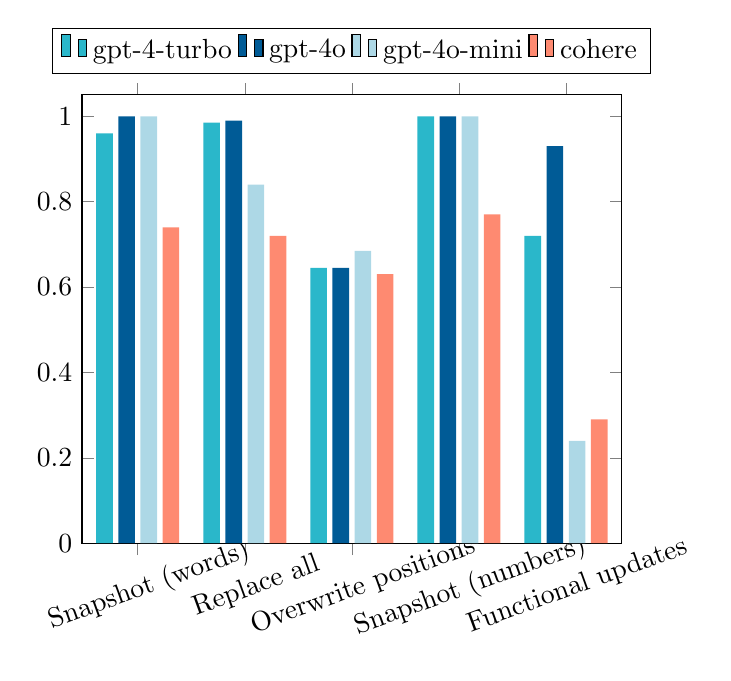
\begin{tikzpicture}
        \begin{axis}[
            ybar,
            bar width=6pt,
            symbolic x coords={Snapshot (words), Replace all, Overwrite positions, Snapshot (numbers), Functional updates},
            xtick=data,
            ymin=0, ymax=1.05,
            legend columns=4,
            legend style={at={(0.5,1.15)}, anchor=north, draw=black},
            enlarge x limits=0.13,
            xticklabel style={rotate=20, anchor=center, yshift=-12pt}
        ]
        
        \addplot[fill={rgb,255:red,42;green,183;blue,202}, draw=none] coordinates {(Snapshot (words),0.96) (Replace all,0.985) (Overwrite positions,0.645) (Snapshot (numbers),1.00) (Functional updates,0.72)};
        \addlegendentry{gpt-4-turbo}
        
        \addplot[fill={rgb,255:red,0;green,91;blue,150}, draw=none] coordinates {(Snapshot (words),1.00) (Replace all,0.99) (Overwrite positions,0.645) (Snapshot (numbers),1.00) (Functional updates,0.93)};
        \addlegendentry{gpt-4o}
        
        \addplot[fill={rgb,255:red,173;green,216;blue,230}, draw=none] coordinates {(Snapshot (words),1.00) (Replace all,0.84) (Overwrite positions,0.685) (Snapshot (numbers),1.00) (Functional updates,0.24)};
        \addlegendentry{gpt-4o-mini}
        
        \addplot[fill={rgb,255:red,254;green,138;blue,113}, draw=none] coordinates {(Snapshot (words),0.74) (Replace all,0.72) (Overwrite positions,0.63) (Snapshot (numbers),0.77) (Functional updates,0.29)};
        \addlegendentry{cohere}
        
        \end{axis}
\end{tikzpicture}}
    \end{subfigure}
    \begin{subfigure}{0.49\columnwidth}
        \resizebox{\textwidth}{!}{    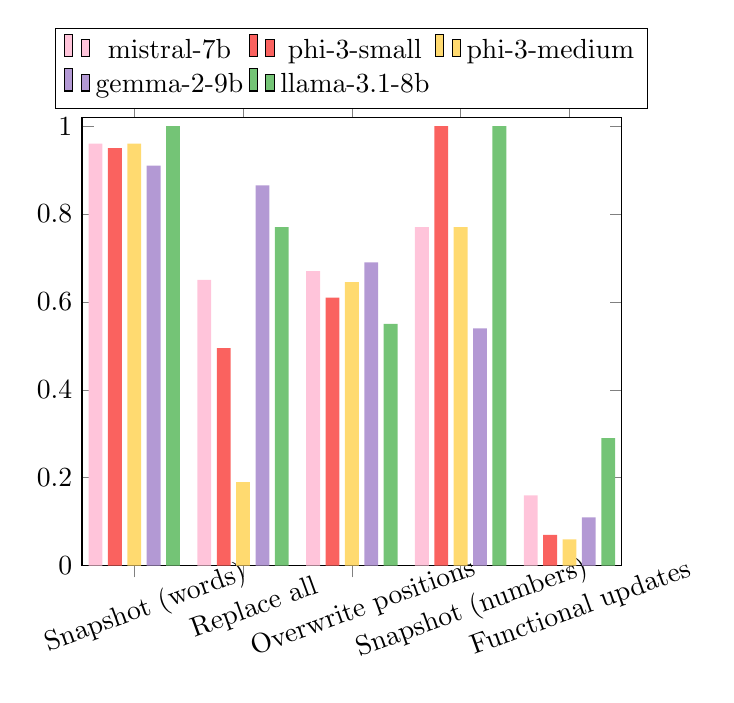
\begin{tikzpicture}
        \begin{axis}[
            ybar,
            bar width=5pt,
            symbolic x coords={Snapshot (words), Replace all, Overwrite positions, Snapshot (numbers), Functional updates},
            xtick=data,
            ymin=0, ymax=1.02,
            legend columns=3,
            legend style={at={(0.5,1.20)}, anchor=north, draw=black},
            enlarge x limits=0.12,
            xticklabel style={rotate=20, anchor=center, yshift=-12pt}
        ]
        
        \addplot[fill={rgb,255:red,255;green,196;blue,218}, draw=none] coordinates {(Snapshot (words),0.96) (Replace all,0.65) (Overwrite positions,0.67) (Snapshot (numbers),0.77) (Functional updates,0.16)};
        \addlegendentry{mistral-7b}
        
        \addplot[fill={rgb,255:red,250;green,98;blue,95}, draw=none] coordinates {(Snapshot (words),0.95) (Replace all,0.495) (Overwrite positions,0.61) (Snapshot (numbers),1.00) (Functional updates,0.07)};
        \addlegendentry{phi-3-small}
        
        \addplot[fill={rgb,255:red,255;green,218;blue,112}, draw=none] coordinates {(Snapshot (words),0.96) (Replace all,0.19) (Overwrite positions,0.645) (Snapshot (numbers),0.77) (Functional updates,0.06)};
        \addlegendentry{phi-3-medium}
        
        \addplot[fill={rgb,255:red,179;green,153;blue,212}, draw=none] coordinates {(Snapshot (words),0.91) (Replace all,0.865) (Overwrite positions,0.69) (Snapshot (numbers),0.54) (Functional updates,0.11)};
        \addlegendentry{gemma-2-9b}
        
        \addplot[fill={rgb,255:red,116;green,196;blue,118}, draw=none] coordinates {(Snapshot (words),1.00) (Replace all,0.77) (Overwrite positions,0.55) (Snapshot (numbers),1.00) (Functional updates,0.29)};
        \addlegendentry{llama-3.1-8b}
        
        \end{axis}
\end{tikzpicture}}
    \end{subfigure}
    \caption{Results for the \textbf{Recall and Edit} tasks.}
    \label{fig:recall}
\end{figure}

\paragraph{Recall and Edit} 
\begin{table}[!h]
    \centering
        \resizebox{0.8\columnwidth}{!}{%
    \begin{tabular}{lllll}
    \toprule
        \textbf{Model} & \textbf{String Search (word)} & \textbf{Snapshot} \\ \hline
gpt-4-turbo    & 1.00 \textcolor{green}{(0.06)} & 1.00 \textcolor{green}{(0.04)} \\ 
gpt-4o         & 1.00 (0.00)                   & 1.00 (0.00)                   \\ 
gpt-4o-mini    & 0.94 \textcolor{red}{(-0.04)}  & 1.00 (0.00)                   \\ 
cohere         & 1.00 (0.00)                   & 1.00 \textcolor{green}{(0.26)} \\ 
mistral-7b     & 1.00 \textcolor{green}{(0.22)} & 0.96 (0.00)                   \\ 
phi-3-small    & 1.00 \textcolor{green}{(0.06)} & 0.99 \textcolor{green}{(0.04)} \\ 
phi-3-medium   & 0.98 \textcolor{red}{(-0.02)}  & 0.87 \textcolor{red}{(-0.09)}  \\ 
gemma-2-9b     & 0.96 \textcolor{red}{(-0.04)}  & 0.96 \textcolor{green}{(0.05)} \\ 
llama-3.1-8b   & 0.98 \textcolor{red}{(-0.02)}  & 1.00 (0.00)                   \\
\bottomrule
    \end{tabular}
    }
    \caption{Ablation study with gibberish context.}
    \label{tab:ablation_gibberish}
\end{table}

Figure \ref{fig:recall} presents the results for the \textbf{Recall and Edit} tasks. While models performed well on basic recall (\textit{Snapshot}), their performance dropped sharply when tasked with making regular edits. A closer analysis of the generated outputs reveals that models struggled with maintaining coherence during edits, often getting trapped in repetitive word loops. For the \textit{Functional Update} task, we deliberately selected simple numerical updates, such as ``Subtract 1 from every number," to ensure the edits were within the models' capabilities. Nevertheless, when comparing performance on \textit{Snapshot (with numbers)} to \textit{Functional Updates}, all models exhibited a steep decline, especially for smaller ones. Analysis of generated outputs revealed that these models frequently deviated from instructions over longer sequences, suggesting difficulties in maintaining consistent rule applications over extended contexts.

Additionally, we conducted a separate ablation study on \textit{Snapshot} and \textit{String Search}. In this study, we replaced meaningful words in the context with gibberish tokens consisting of randomly generated alphabetical characters. As shown in Table \ref{tab:ablation_gibberish}, performance remained largely unchanged, suggesting that semantic meaning was not a significant distractor in these tasks.

\begin{table}
\centering
% \footnotesize
\resizebox{\linewidth}{!}{
\setlength{\tabcolsep}{5pt}
\begin{tabular}[t]{l|ccc}
\toprule
 \makecell[c]{\textbf{Method}} & \makecell[c]{\textbf{Self}\\\textbf{Reflection}} & \makecell[c]{\textbf{Memory}} & \makecell[c]{\textbf{Length}\\\textbf{Generalization}} \\
\midrule
Revision~\cite{DBLP:journals/corr/abs-2408-03314} & \redcross & \greencheck & \redcross \\
Self-Refine~\cite{DBLP:conf/nips/MadaanTGHGW0DPY23} & \greencheck & \greencheck & \redcross \\
Best-of-N~\cite{DBLP:journals/corr/abs-2407-21787} & \redcross & \redcross & \greencheck \\
Beam Search~\cite{ow1988filtered} & \redcross & \redcross & \greencheck \\
Guided Beam Search~\cite{DBLP:conf/nips/XieKZZKHX23} & \greencheck & \redcross & \greencheck \\
\midrule
\textbf{FTTT (ours)} & \greencheck & \greencheck & \greencheck \\
\bottomrule
\end{tabular}
}
% \vspace{-5pt}
\caption{Comparing the advantages and drawbacks of FTTT and related works.}
\label{tab:compare}
% \vspace{-0.5cm}
\end{table}

\begin{table}[!htbp] \centering
  \caption{Human Choices and Predictions About GenAI Choice in the Same Problem: Heterogeneity by Exposure and Attitudes (Pooled)}
\begin{adjustbox}{scale=0.8}
\begin{tabular}{@{\extracolsep{5pt}}lccccc}
% \\[-1.8ex]\hline
% \hline \\[-1.8ex]
\toprule
& \multicolumn{5}{c}{\textit{Dependent variable: Prediction}} \
\cr \cline{2-6}
\\[-1.8ex] & \multicolumn{1}{c}{Heavy User} & \multicolumn{1}{c}{Text-Based LLM User} & \multicolumn{1}{c}{Paid User} & \multicolumn{1}{c}{Agree AI Similar} & \multicolumn{1}{c}{Agree AI Better}  \\
\\[-1.8ex] & (1) & (2) & (3) & (4) & (5) \\
% \hline \\[-1.8ex]
\midrule
 X$\times$Heavy User & -0.056$^{}$ & & & & \\
& (0.052) & & & & \\
 X$\times$Text-Based LLM User & & 0.082$^{**}$ & & & \\
& & (0.040) & & & \\
 X$\times$Paid User & & & -0.001$^{}$ & & \\
& & & (0.072) & & \\
 X$\times$Agree AI Similar & & & & 0.033$^{}$ & \\
& & & & (0.045) & \\
 X$\times$Agree AI Better & & & & & 0.019$^{}$ \\
& & & & & (0.017) \\
 Problem FE & Yes & Yes & Yes & Yes & Yes \\
 X$\times$Problem FE & Yes & Yes & Yes & Yes & Yes \\
 G$\times$Problem FE & Yes & Yes & Yes & Yes & Yes \\
% \hline \\[-1.8ex]
\midrule
 Observations & 2700 & 2700 & 2700 & 2700 & 2700 \\
 % Residual Std. Error & 22.874 & 22.851 & 22.863 & 22.847 & 22.895 \\
% \hline
% \hline \\[-1.8ex]
\bottomrule
\textit{Note:} & \multicolumn{5}{r}{Standard errors are clustered at the problem level. $^{*}$p$<$0.1; $^{**}$p$<$0.05; $^{***}$p$<$0.01} \\
% \multicolumn{6}{r}\textit{} \\
\end{tabular}
\end{adjustbox}
\label{tab:group} \end{table}


\paragraph{Match and Compare}
 As shown in Figure \ref{fig:match}, model performance in the \textbf{Match and Compare} tasks was relatively consistent across different model sizes. Given that counting is a well-known weakness in LLMs, it is unsurprising that all models struggled significantly with the counting task, though GPT models performed slightly better than others. However, models generally succeeded in identifying the duplicates (in \textit{Find duplicates}), and primarily struggled with the counting aspect -- which requires tracking and updating an integer state, a skill that is more similar to stateful processing. This suggests that relying solely on counting-based tests \cite{song2024countingstars} could overly bias the evaluation and fail to capture broader model capabilities. The results also indicate that models exhibit some ability to recognize relative positions and group associations, but their accuracy remains limited (ranging between 0.6-0.8). A closer examination of model generations reveals an overwhelming tendency for the models to produce false positive errors -- models often answer “yes” when the correct answer is “no”, while making very few false negative errors. This means that when the relationship is correct, the models can more reliably identify it. This may stem from a combination of their inherent inclination to agree and the difficulty in recognizing relative comparisons and associations.

% \begin{figure}[h]
%     \centering
%     \includegraphics[width=0.92\columnwidth]{images/difference.png}
%     \caption{Results for \textbf{Spot the Differences }tasks.}
%     \label{fig:difference}
% \end{figure}

\begin{figure}[h]
\centering
\resizebox{0.9\columnwidth}{!}{
 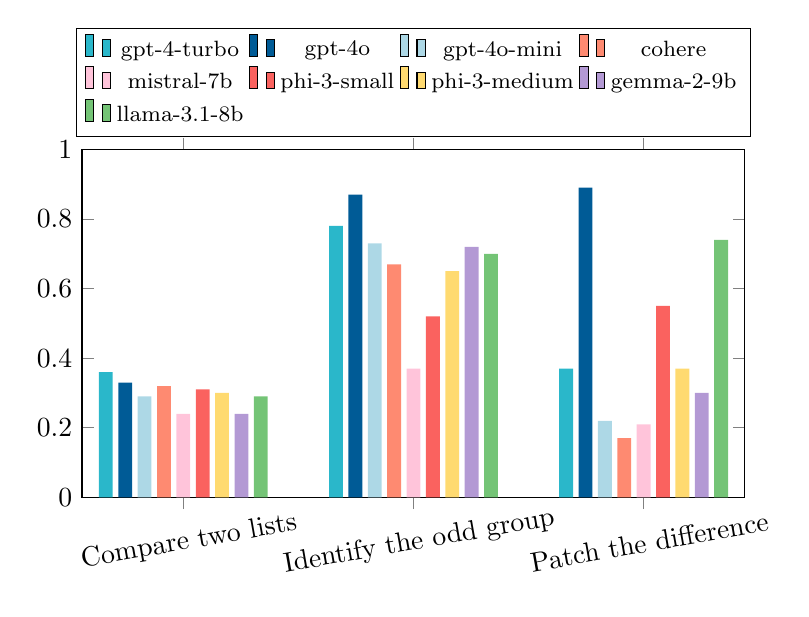
\begin{tikzpicture}
        \begin{axis}[
            ybar,
            bar width=5pt,
            symbolic x coords={Compare two lists, Identify the odd group, Patch the difference},
            xtick=data,
            ymin=0, ymax=1.0,
            legend columns=4,
            legend style={at={(0.5,1.35)}, anchor=north, draw=black, font=\footnotesize},
            enlarge x limits=0.22,
            xticklabel style={rotate=10, anchor=center, yshift=-12pt},
            width=10cm, height=6cm,
        ]
        
        \addplot[fill={rgb,255:red,42;green,183;blue,202}, draw=none] coordinates {(Compare two lists,0.36) (Identify the odd group,0.78) (Patch the difference,0.37)};
        \addlegendentry{gpt-4-turbo}
        
        \addplot[fill={rgb,255:red,0;green,91;blue,150}, draw=none] coordinates {(Compare two lists,0.33) (Identify the odd group,0.87) (Patch the difference,0.89)};
        \addlegendentry{gpt-4o}
        
        \addplot[fill={rgb,255:red,173;green,216;blue,230}, draw=none] coordinates {(Compare two lists,0.29) (Identify the odd group,0.73) (Patch the difference,0.22)};
        \addlegendentry{gpt-4o-mini}
        
        \addplot[fill={rgb,255:red,254;green,138;blue,113}, draw=none] coordinates {(Compare two lists,0.32) (Identify the odd group,0.67) (Patch the difference,0.17)};
        \addlegendentry{cohere}
        
        \addplot[fill={rgb,255:red,255;green,196;blue,218}, draw=none] coordinates {(Compare two lists,0.24) (Identify the odd group,0.37) (Patch the difference,0.21)};
        \addlegendentry{mistral-7b}
        
        \addplot[fill={rgb,255:red,250;green,98;blue,95}, draw=none] coordinates {(Compare two lists,0.31) (Identify the odd group,0.52) (Patch the difference,0.55)};
        \addlegendentry{phi-3-small}
        
        \addplot[fill={rgb,255:red,255;green,218;blue,112}, draw=none] coordinates {(Compare two lists,0.30) (Identify the odd group,0.65) (Patch the difference,0.37)};
        \addlegendentry{phi-3-medium}
        
        \addplot[fill={rgb,255:red,179;green,153;blue,212}, draw=none] coordinates {(Compare two lists,0.24) (Identify the odd group,0.72) (Patch the difference,0.30)};
        \addlegendentry{gemma-2-9b}
        
        \addplot[fill={rgb,255:red,116;green,196;blue,118}, draw=none] coordinates {(Compare two lists,0.29) (Identify the odd group,0.70) (Patch the difference,0.74)};
        \addlegendentry{llama-3.1-8b}
        
        \end{axis}
    \end{tikzpicture}}
    \caption{Results for \textbf{Spot the Differences }tasks.}
    \label{fig:difference}
\end{figure}

\paragraph{Spot the Differences}
As shown in Figure \ref{fig:difference}, performance across all models are poor on \textit{Compare Two Lists}, suggesting inherent difficulties in cross-referencing information across long contexts, even for larger models.  GPT-4o and the LLaMA model significantly outperform the others in the \textit{Identify the Odd Group} task, highlighting a general weakness in detecting contextual differences by the other models. However, an 8B LLaMA model outperforms both equivalently-sized models and even GPT-4 in this task, suggesting that model size alone was not the determining factor. This indicates that architectural differences, training objectives, or specific inductive biases may contribute to improved performance in comparative memory utilization.


\paragraph{Compute on Sets and Lists}
The tasks in this category require models to recognize and process group structures within the context, and performance gradually declines as the complexity of the task increases (see Table \ref{tab:lists}). For instance, in comparing the \textit{Group Membership} task with the \textit{String Search} task, where the former requires identifying which list a word belongs to rather than simply determining its presence, the performance of open-source models drops considerably. Similarly, in comparing the \textit{Group Association} task with the \textit{Group Membership} task, where the former requires determining whether two words belong to the same group, all models exhibit a noticeable decline in performance. The decline becomes even more pronounced when comparing the \textit{ Group Association (alternating)} variant of the task to the standard \textit{Group Association} task. Here, the context involves alternating repeated groups rather than simple group structures, which further challenges the models' abilities to handle partitioned contexts effectively.

An interesting observation was found during the \textit{Iterate} task. In an ablation study, we modified the task to require returning the first words in each list instead of the last words (making it more similar to the \textit{Batch Search} task). The performance sharply declines when models are asked to return the last words, despite their strong information-fetching capabilities. This suggests that, while the models can retrieve information effectively, they struggle to accurately recognize and process partitions within the context.



\begin{table}[t!]
\centering
    \resizebox{0.7\columnwidth}{!}{%

\begin{tabular}{lcc}
\toprule
\textbf{Model} & \textbf{Quantity state} & \textbf{Set state} \\
\midrule
gpt-4-turbo & 0.8 & \textbf{0.80} \\
gpt-4o & \textbf{1.0} & 0.65 \\
gpt-4o-mini & 0.7 & 0.24 \\
cohere & 0.0 & 0.58 \\
mistral-7b & 0.0 & 0.08 \\
phi-3-small & 0.0 & 0.13 \\
phi-3-medium & 0.0 & 0.11 \\
gemma-2-9b & 0.0 & 0.24 \\
llama-3.1-8b & 0.0 & 0.13 \\
\bottomrule
\end{tabular}
}
\caption{Results for \textbf{Stateful Processing} tasks.}
\label{tab:state}
\end{table}
\paragraph{Stateful Processing}

\begin{figure}[t!]
    \centering
    \begin{subfigure}{0.49\columnwidth}
        \resizebox{\textwidth}{!}{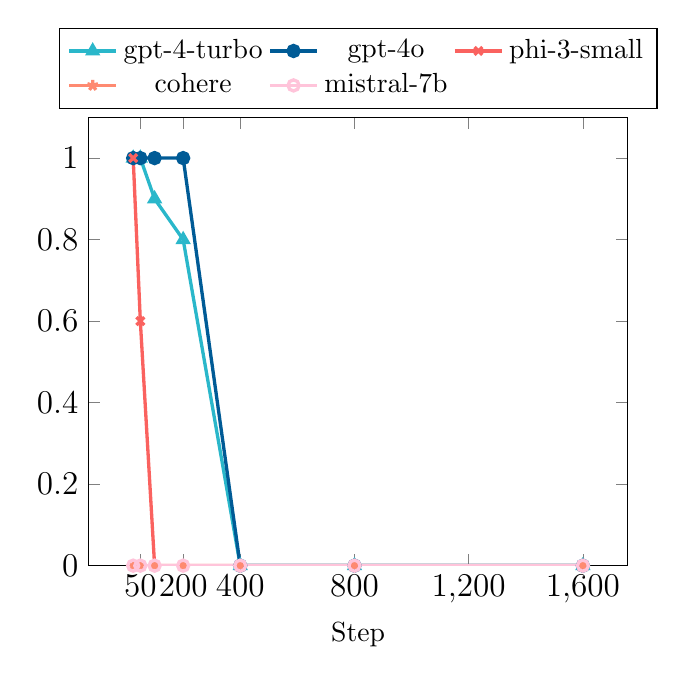
\begin{tikzpicture}
    \begin{axis}[
        xlabel={Step},
        legend style={at={(0.5,1.2)}, anchor=north, cells={align=left}, legend columns=3},
        ymin=0, ymax=1.1,
        xtick={50, 200, 400, 800, 1200, 1600},
        ytick={0,0.2,0.4,0.6,0.8,1.0},
        grid=none,
        tick label style={font=\large}
    ]

    % GPT-4-Turbo
    \addplot[mark=triangle, very thick, color={rgb,255:red,42;green,183;blue,202}] coordinates {
        (25,1.0) (50,1.0) (100,0.9) (200,0.8) (400,0.0) (800,0.0) (1600,0.0)
    };
    \addlegendentry{gpt-4-turbo}

    % GPT-4o
    \addplot[mark=*, very thick, color={rgb,255:red,0;green,91;blue,150}] coordinates {
        (25,1.0) (50,1.0) (100,1.0) (200,1.0) (400,0.0) (800,0.0) (1600,0.0)
    };
    \addlegendentry{gpt-4o}



    % Phi-3-Small
    \addplot[mark=x, very thick, color={rgb,255:red,250;green,98;blue,95}] coordinates {
        (25,1.0) (50,0.6) (100,0.0) (200,0.0) (400,0.0) (800,0.0) (1600,0.0)
    };
    \addlegendentry{phi-3-small}

    % Cohere
    \addplot[mark=star, very thick, color={rgb,255:red,254;green,138;blue,113}] coordinates {
        (25,0.0) (50,0.0) (100,0.0) (200,0.0) (400,0.0) (800,0.0) (1600,0.0)
    };
    \addlegendentry{cohere}

    % Mistral-7B
    \addplot[mark=o, very thick, color={rgb,255:red,255;green,196;blue,218}] coordinates {
        (25,0.0) (50,0.0) (100,0.0) (200,0.0) (400,0.0) (800,0.0) (1600,0.0)
    };
    \addlegendentry{mistral-7b}
    
    \end{axis}
\end{tikzpicture}}
    \end{subfigure}
    \begin{subfigure}{0.49\columnwidth}
        \resizebox{\textwidth}{!}{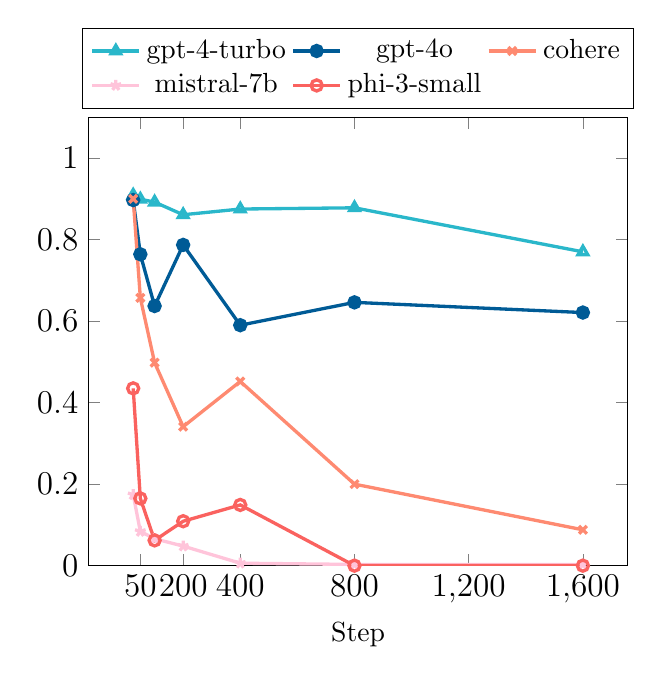
\begin{tikzpicture}
    \begin{axis}[
        xlabel={Step},
        legend style={at={(0.5,1.2)}, anchor=north, cells={align=left}, legend columns=3},
        ymin=0, ymax=1.1,
        xtick={50, 200, 400, 800, 1200, 1600},
        ytick={0,0.2,0.4,0.6,0.8,1.0},
        grid=none,
        tick label style={font=\large}
    ]

    % GPT-4-Turbo
    \addplot[mark=triangle, very thick, color={rgb,255:red,42;green,183;blue,202}] coordinates {
        (25,0.909) (50,0.899) (100,0.892) (200,0.861) (400,0.875) (800,0.878) (1600,0.770)
    };
    \addlegendentry{gpt-4-turbo}

    % GPT-4o
    \addplot[mark=*, very thick, color={rgb,255:red,0;green,91;blue,150}] coordinates {
        (25,0.897) (50,0.764) (100,0.637) (200,0.787) (400,0.590) (800,0.646) (1600,0.621)
    };
    \addlegendentry{gpt-4o}

    % Cohere
    \addplot[mark=x, very thick, color={rgb,255:red,254;green,138;blue,113}] coordinates {
        (25,0.900) (50,0.657) (100,0.498) (200,0.341) (400,0.452) (800,0.200) (1600,0.088)
    };
    \addlegendentry{cohere}

    % Mistral-7B
    \addplot[mark=star, very thick, color={rgb,255:red,255;green,196;blue,218}] coordinates {
        (25,0.174) (50,0.084) (100,0.066) (200,0.048) (400,0.006) (800,0.003) (1600,0.003)
    };
    \addlegendentry{mistral-7b}

    % Phi-3-Small
    \addplot[mark=o, very thick, color={rgb,255:red,250;green,98;blue,95}] coordinates {
        (25,0.435) (50,0.165) (100,0.062) (200,0.109) (400,0.149) (800,0.000) (1600,0.000)
    };
    \addlegendentry{phi-3-small}
    
    \end{axis}
\end{tikzpicture}}
    \end{subfigure}
    \caption{Ablation study on the number of operation steps for the \textbf{quantity state} (left) and\textbf{ set state }(right).}
    \label{fig:ablation_state_step}
\end{figure}



Table \ref{tab:state} presents the results for the \textbf{Stateful Processing} tasks, where performance gaps among models are the most pronounced. The GPT-4(o) models perform well on integer state tracking, while most other models struggle (near zero accuracy). For set state tracking, larger models generally perform better.

We conducted an ablation study to examine how the number of operation steps influences performance of five selected models (Fig. \ref{fig:ablation_state_step}). For quantity state tracking, GPT-4(o) models perform well within fewer than 200 steps but experience a sharp decline in accuracy beyond this threshold. For set state tracking, the performance decline is more gradual. The differences in performance drop between the two tasks can be attributed to the nature of the two tasks. While tracking an integer state might seem simpler than tracking a set, it actually requires the model to maintain and apply every operation sequentially to compute the final value. In contrast, for set state, the fixed size of the set makes more recent operations more relevant to the final state, reducing the need for exhaustive step-by-step tracking. Nevertheless, even in this scenario, all models show a clear inability to handle longer or more complex operation sequences effectively. Interestingly, GPT-4 model outperformed GPT-4o at this task, suggesting potential optimization trade-offs may have affected its ability to manage set-based updates. 

Overall, while larger models like GPT-4(o) exhibit some ability to track state over time, their effectiveness rapidly deteriorates as task complexity increases. Smaller models, in particular, struggle to track operations over time, pointing to significant gaps in their ability to manage and process sequential dependencies critical for state tracking tasks.

\subsection{Results on Composite Tests}

\section{Simple Construction of Projective Compositions}
\label{sec:comp_coord}

It is not clear apriori that projective compositional distributions satisfying Definition \ref{def:proj_comp} ever exist, much less that there is any straightforward way to sample from them.
To explore this, we first restrict attention to perhaps the simplest setting, where the projection functions $\{\Pi_i\}$ are
just coordinate restrictions.
This setting is meant to generalize the intuition we had
in the CLEVR example of Figure~\ref{fig:len_gen},
where different objects were composed in disjoint regions of the image.
We first define the construction of the composed distribution,
and then establish its theoretical properties.








\subsection{Defining the Construction}
Formally, suppose we have a set of distributions
$(p_1, p_2, \ldots, p_k)$ that we wish to compose;
in our running CLEVR example, each $p_i$ is the distribution of images
with a single object at position $i$.
Suppose also we have some reference distribution $p_b$,
which can be arbitrary, but should be thought of as a 
``common background'' to the $p_i$s.
Then, one popular way to construct a composed distribution
is via the \emph{compositional operator} defined below.
(A special case of this construction is used in \citet{du2023reduce}, for example).


\begin{definition}[Composition Operator]
    \label{def:comp_oper}
    Define the \emph{composition operator} $\cC$ acting on an arbitrary set of distributions $(p_b, p_1, p_2, \ldots)$ by
    \begin{align}
    \label{eq:comp_oper}
    \cC[\vec{p}] := \cC[p_b, p_1, p_2, \dots](x) := \frac{1}{Z} p_b(x) \prod_i \frac{p_i(x)}{p_b(x)},
    \end{align}
    where $Z$ is the appropriate normalization constant. We name $\cC[\vec{p}]$ the \emph{composed distribution}, and the score of $\cC[\vec{p}]$ the \emph{compositional score}:
    \begin{align}
    \label{eqn:comp_score}
    &\grad_x \log \cC[\vec{p}](x)  \\
    &= \grad_x \log p_b(x) + \sum_i \left( \grad_x \log p_i(x) - \grad_x \log p_b(x) \right). \notag
    \end{align}
\end{definition}
Notice that if $p_b$ is taken to be the unconditional distribution then this is exactly the Bayes-composition.


\vspace{-0.5em}
\subsection{When does the Composition Operator Work?}
We can always apply the composition operator to any set of distributions,
but when does this actually yield a ``correct'' composition
(according to Definition~\ref{def:proj_comp})?
One special case is when each distribution $p_i$ is
``active'' on a different, non-overlapping set of coordinates.
We formalize this property below
as \emph{Factorized Conditionals} (Definition~\ref{def:factorized}).
The idea is, 
each distribution $p_i$
must have a particular set of ``mask'' coordinates $M_i \subseteq [n]$ which it
samples in a characteristic way,
while independently sampling all other coordinates
from a common background distribution.
If a set of distributions $(p_b, p_1, p_2, \ldots)$ has this
\emph{Factorized Conditional} structure, then 
the composition
operator will produce a projective composition (as we will prove below).



\begin{definition}[Factorized-Conditionals]
\label{def:factorized}

We say a set of distributions $(p_b, p_1, p_2, \dots p_k)$
over $\R^n$
are \emph{Factorized Conditionals} if
there exists a partition of coordinates $[n]$
into disjoint subsets $M_b, M_1, \dots M_k$ such that:
\begin{enumerate}
    \setlength{\itemsep}{1pt}
    \item $(x|_{M_i}, x|_{M_i^c})$ are independent under $p_i$.
    \item $(x|_{M_b}, x|_{M_1}, x|_{M_2}, \dots, x|_{M_k})$
    are mutually independent under $p_b$.
    \item $p_i(x|_{M_i^c}) = p_b(x|_{M_i^c})$.
\end{enumerate}

Equivalently, if we have:
\begin{align}
    p_i(x) &= p_i(x|_{M_i}) p_b(x|_{M_i^c}), \text{ and} \label{eqn:cc-cond}\\
    p_b(x) &= p_b(x|_{M_b}) \prod_{i \in [k]} p_b(x|_{M_i}). \notag
\end{align}
\end{definition}
\vspace{-1em}
Equation~\eqref{eqn:cc-cond} means that each $p_i$
can be sampled by first sampling $x \sim p_b$,
and then overwriting the coordinates of $M_i$
according to some other distribution (which can be specific to distribution $i$).
For instance, the experiment of Figure~\ref{fig:len_gen}
intuitively satisfies this property, since 
each of the conditional distributions could essentially be sampled
by first sampling an empty background image ($p_b$), then ``pasting''
a random object in the appropriate location (corresponding to pixels $M_i$).
If a set of distributions obey this Factorized Conditional structure,
then we can prove that the composition operator $\cC$
yields a correct projective composition,
and reverse-diffusion correctly samples from it.
Below, let $N_t$ denote the noise operator of the
diffusion process\footnote{Our results are agnostic to the specific diffusion noise-schedule and scaling used.} at time $t$.

\begin{theorem}[Correctness of Composition]
\label{lem:compose}
Suppose a set of distributions $(p_b, p_1, p_2, \dots p_k)$
satisfy Definition~\ref{def:factorized},
with corresponding masks $\{M_i\}_i$.
Consider running the reverse-diffusion SDE 
using the following compositional scores at each time $t$:
\begin{align}
s_t(x_t) &:= \grad_x \log \cC[p_b^t, p_1^t, p_2^t, \ldots](x_t),
\end{align}
where $p_i^t := N_t[p_i]$ are the noisy distributions.
Then, the distribution of the generated sample $x_0$ at time $t=0$ is:
\begin{align}
\label{eqn:p_hat}
\hat{p}(x) := p_b(x|_{M_b}) \prod_i p_i(x|_{M_i}).
\end{align}
In particular,
$\hat{p}(x|_{M_i}) = p_i(x|_{M_i})$ for all $i$,
and so
$\hat{p}$ is a projective composition
with respect to projections $\{\Pi_i(x) := x|_{M_i}\}_i$,
per Definition \ref{def:proj_comp}.
\end{theorem}




Unpacking this, Line \ref{eqn:p_hat} says that the final generated distribution
$\hat{p}(x)$ can be sampled by
first sampling
the coordinates $M_b$ according to $p_b$ (marginally),
then independently sampling 
coordinates $M_i$ according to $p_i$ (marginally) for each $i$.
Similarly, by assumption, $p_i(x)$ can be sampled by first sampling the coordinates $M_i$ in some specific way, and then independently sampling the remaining coordinates according to $p_b$. Therefore Theorem \ref{lem:compose} says that $\hat{p}(x)$ samples the coordinates \emph{$M_i$ exactly as they would be sampled by $p_i$}, for each $i$ we wish to compose. 

\begin{proof}(Sketch) \small
Since $\vec{p}$ satisfies Definition \ref{def:factorized}, we have
\begin{align*}
&\cC[\vec{p}](x) := p_b(x) \prod_i \frac{p_i(x)}{p_b(x)} \notag 
= p_b(x) \prod_i \frac{p_b(x_t|_{M_i^c}) p_i(x|_{M_i})}{p_b(x|_{M_i^c})p_b(x|_{M_i})} \notag \\
&= p_b(x) \prod_i \frac{p_i(x|_{M_i})}{p_b(x|_{M_i})} \notag 
= p_b(x|_{M_b}) \prod_i p_i(x_t|_{M_i}) := \hat{p}(x).
\end{align*}
The sampling guarantee follows from the commutativity of composition with the diffusion noising process, i.e. $\cC[\vec{p^t}]= N_t[\cC[\vec{p}]]$. 
The complete proof is in Appendix \ref{app:compose_pf}.
\end{proof}

\begin{remark}
In fact, Theorem~\ref{lem:compose} still holds under any orthogonal transformation of the variables,
because the diffusion noise process commutes with orthogonal transforms.
We formalize this as Lemma~\ref{lem:orthogonal_sampling}.
\end{remark}

\begin{remark}
Compositionality is often thought of in terms of orthogonality between scores.
Definition \ref{def:factorized} implies orthogonality between the score differences that appear in the composed score \eqref{eqn:comp_score}:
$\grad_x \log p_i^t(x_t) - \grad_x \log p_b^t(x_t),$
but the former condition is strictly stronger
(c.f. Appendix \ref{app:score_orthog}).
\end{remark}

\begin{remark}
Notice that the composition operator $\cC$
can be applied to a set of Factorized Conditional
distributions
without knowing the coordinate partition $\{M_i\}$.
That is, we can compose distributions and compute scores
without knowing apriori exactly ``how'' these distributions are supposed to compose
(i.e. which coordinates $p_i$ is active on).
This is already somewhat remarkable, and we will see a much
stronger version of this property in the next section.
\end{remark}

\textbf{Importance of background.}
Our derivations highlight the crucial role of the background
distribution $p_b$ for the composition operator  
(Definition~\ref{def:comp_oper}).
While prior works have taken $p_b$ to be an unconditional distribution and the $p_i$'s its associated conditionals,
our results suggest this is not always the optimal choice -- in particular,
it may not satisfy a Factorized Conditional structure (Definition~\ref{def:factorized}). Figure~\ref{fig:len_gen_monster} demonstrates this empirically: settings (a) and (b) attempt to compose the same distributions using different backgrounds -- empty (a) or unconditional (b) -- with very different results.

\subsection{Approximate Factorized Conditionals in CLEVR.}
\label{sec:clevr-details}

In \cref{fig:len_gen_monster} we explore compositional length-generalization (or lack thereof) in three different setting, two of which (\cref{fig:len_gen_monster}a and \ref{fig:len_gen_monster}c) approximately satisfy \cref{def:factorized}. In this section we explicitly describe how our definition of Factorized Conditionals approximately captures the CLEVR settings of Figures \ref{fig:len_gen_monster}a and \ref{fig:len_gen_monster}c. The setting of \ref{fig:len_gen_monster}b does not satisfy our conditions, as discussed in \cref{sec:problematic-compositions}.

\textbf{Single object distributions with empty background.}
This is the setting of both \cref{fig:len_gen} and \cref{fig:len_gen_monster}a.
The background distribution $p_b$ 
over $n$ pixels is images of an empty scene with no objects.
For each $i \in \{1,\ldots,L\}$ (where $L=4$ in \cref{fig:len_gen} and $L=9$ in \cref{fig:len_gen_monster}a), define the set $M_i \subset [n]$ 
as the set of pixel indices surrounding location $i$.
($M_i$ should be thought of as a ``mask'' that
that masks out objects at location $i$).
Let $M_b := (\cup_i M_i)^c$ be the remaining
pixels in the image.
Then, we claim the distributions $(p_b, p_1, \ldots, p_L)$
form approximately
Factorized Conditionals, with corresponding
coordinate partition $\{M_i\}$.
This is essentially because each distribution $p_i$
matches the background $p_b$ on all pixels except those surrounding
location $i$ (further detail in Appendix~\ref{app:clevr-details}).
Note, however, that the conditions of Definition~\ref{def:factorized}
do not \emph{exactly} hold in the experiment of Figure~\ref{fig:len_gen} -- there is still some dependence between
the masks $M_i$, since objects can cast shadows or even occlude each other.
Empirically, these deviations 
have greater impact
when composing many objects, as seen in \cref{fig:len_gen_monster}a.


\textbf{Bayes composition with cluttered distributions.}
In \cref{fig:len_gen_monster}c we replicate CLEVR experiments in  \citet{du2023reduce, liu2022compositional} where the images contain many objects (1-5) and the conditions label the location of one randomly-chosen object. It turns out the unconditional together with the conditionals can approximately act as Factorized Conditionals in ``cluttered'' settings like this one. The intuition is that if the conditional distributions each contain one specific object plus many independently sampled random objects (``clutter''), then the unconditional distribution \emph{almost} looks like independently sampled random objects, which together with the conditionals \emph{would} satisfy Definition \ref{def:factorized} (further discussion in Appendix \ref{app:clevr-details} and \ref{app:bayes_connect}). This helps to explain the length-generalization observed in \citet{liu2022compositional} and verified in our experiments (\cref{fig:len_gen_monster}c).







\section{Projective Composition in Feature Space}
\label{sec:comp_feature}

\begin{figure}
    \centering
    \includegraphics[width=1.0\linewidth]{figures/feat-space-vis.png}
    \caption{A commutative diagram illustrating Theorem~\ref{lem:transform_comp}.
    Performing composition in pixel space is equivalent 
    to encoding into a feature space ($\cA$),
    composing there,
    and decoding back
    to pixel space ($\cA^{-1}$).
    }
    \label{fig:feat-space-vis}
\end{figure}

So far we have focused on the setting where the projection functions $\Pi_i$ are simply projections onto coordinate subsets $M_i$ in the native space (e.g. pixel space).
This covers simple examples like Figure~\ref{fig:len_gen} but does not include more realistic situations such as Figure~\ref{fig:style-content},
where the properties to be composed are more abstract.
For example a property like ``oil painting'' does not correspond to projection
onto a specific subset of pixels in an image.
However, we may hope that there exists some conceptual feature space
in which ``oil painting'' does correspond to a particular subset of variables.
In this section, we extend our results to the case where the composition occurs in some conceptual feature space, and each distribution to be composed
corresponds to some particular subset of \emph{features}.


Our main result is a featurized analogue of Theorem~\ref{lem:compose}:
if there exists \emph{any} invertible transform $\cA$
mapping into a feature space
where Definition \ref{def:factorized} holds,
then the composition operator (Definition~\ref{def:comp_oper})
yields a projective composition in this feature space, as shown in Figure~\ref{fig:feat-space-vis}.

\begin{theorem}[Feature-space Composition]
\label{lem:transform_comp}
Given distributions $\vec{p} := (p_b, p_1, p_2, \dots p_k)$,
suppose there exists a diffeomorphism $\cA: \R^n \to \R^n$
such that
$(\cA \sharp p_b, \cA \sharp p_1, \dots \cA \sharp p_k)$
satisfy Definition~\ref{def:factorized},
with corresponding partition $M_i \subseteq [n]$.
Then, the composition $\hat{p} := \cC[\vec{p}]$ satisfies:
\begin{align}
\label{eqn:p_hat_A}
\cA \sharp \hat{p}(z)
\equiv
(\cA \sharp p_b (z))|_{M_b} \prod_{i=1}^k (\cA \sharp p_i(z))|_{M_i}.
\end{align}
Therefore, $\hat{p}$
is a projective composition of $\vec{p}$ w.r.t. projection functions
$\{\Pi_i(x) := \cA(x)|_{M_i}\}$.
\end{theorem}
This theorem is remarkable because it means we can
compose distributions $(p_b, p_1, p_2, \dots)$ in the base space,
and this composition will ``work correctly'' in the feature space
automatically (Equation~\ref{eqn:p_hat_A}),
without us ever needing to compute or even know the feature transform $\cA$
explicitly.



Theorem~\ref{lem:transform_comp} may apriori seem too strong
to be true, since it somehow holds for all feature spaces $\cA$
simultaneously.
The key observation underlying Theorem~\ref{lem:transform_comp} 
is that the composition operator $\cC$ behaves
well under reparameterization.
\begin{lemma}[Reparameterization Equivariance]
\label{lem:reparam}
The composition operator of Definition~\ref{def:comp_oper}
is reparameterization-equivariant. That is,
for all diffeomorphisms $\cA: \R^n \to \R^n$
and all tuples of distributions $\vec{p} = (p_b, p_1, p_2, \dots, p_k)$,
\begin{align}
 \cC[ \cA \sharp \vec{p}] =  \cA \sharp \cC[\vec{p}].
\end{align}
\end{lemma}
\arxiv{\footnote{
For example (separate from our goals in this paper):
Classifier-Free-Guidance can be seen as an instance of the composition operator.
Thus, Lemma~\ref{lem:reparam} implies that performing CFG
in latent space is \emph{equivalent} to CFG in pixel-space,
assuming accurate score-models in both cases.}}
\arxiv{This lemma is potentially of independent interest:
reparametrization-equivariance
is a very strong property which is typically not satisfied by
standard operations between probability distributions---
for example, the ``simple product'' $p_1(x)p_2(x)$ does not satisfy it---
so it is mathematically notable that the composition operator 
has this structure.
Lemma~\ref{lem:reparam} and Theorem~\ref{lem:transform_comp}
are proved in Appendix \ref{app:param-indep}.}

This lemma is potentially of independent interest:
equivariance distinguishes the composition operator
from many other common operators
(e.g. the simple product).
Lemma ~\ref{lem:reparam} and Theorem~\ref{lem:transform_comp}
are proved in Appendix \ref{app:param-indep}.

\section{Sampling from Compositions.}
The feature-space Theorem~\ref{lem:transform_comp} is weaker than Theorem~\ref{lem:compose}
in one important way: it does not provide a sampling algorithm.
That is, Theorem~\ref{lem:transform_comp} guarantees that $\hat{p} := \cC[\vec{p}]$
is a projective composition, but does not guarantee that reverse-diffusion
is a valid sampling method.

There is one special case where diffusion sampling \emph{is} guaranteed to work, namely, for orthogonal transforms (which can seen as a straightforward extension of the coordinate-aligned case of \cref{lem:compose}):
\begin{lemma}[Orthogonal transform enables diffusion sampling]
\label{lem:orthogonal_sampling}
If the assumptions of Lemma \ref{lem:transform_comp} hold for $\cA(x) = Ax$, where $A$ is an orthogonal matrix, then running a reverse diffusion sampler with scores $s_t = \grad_x \log \cC[\vec{p}^t]$ generates the composed distribution $\hat{p} = \cC[\vec{p}]$ satisfying \eqref{eqn:p_hat_A}.
\end{lemma}
The proof is given in \cref{app:orthog_sample_pf}.

However, for general invertible transforms, we have no such sampling guarantees.
Part of this is inherent: in the feature-space setting, the 
diffusion noise operator $N_t$ no longer commutes
with the composition operator $\cC$ in general,
 so scores of the noisy composed 
distribution $N_t[\cC[\vec{p}]]$
cannot be computed from scores
of the noisy base distributions $N_t[\vec{p}]$.
Nevertheless, one may hope to sample from the distribution $\hat{p}$
using other samplers besides diffusion, 
such as annealed Langevin Dynamics
or
Predictor-Corrector methods \citep{song2020score}.
We find that the situation is surprisingly subtle:
composition $\cC$ produces distributions which
are in some cases easy to sample (e.g. with diffusion),
yet in other cases apparently hard to sample.
For example, in the
setting of Figure~\ref{fig:clevr_color_comp}, 
our Theorem~\ref{lem:transform_comp} implies
that all pairs of colors should compose equally well
at time $t=0$, since there exist diffeomorphisms
(indeed, linear transforms) between different colors.
However, as we saw,
the diffusion sampler
fails to sample from compositions 
of non-orthogonal colors--- and 
empirically, even more sophisticated
samplers such as Predictor-Correctors
also fail in this setting.
At first glance, it may seem odd that
composed distributions are so hard to sample,
when their constituent distributions are relatively easy to sample.
One possible reason for this below is that the composition operator has extremely poor Lipchitz constant,
so it is possible for a set of distributions $\vec{p}$ to ``vary smoothly''
(e.g. diffusing over time) while their composition $\cC[\vec{p}]$
changes abruptly.
We formalize this in \cref{lem:lipschitz} (further discussion and proof in Appendix \ref{app:lipschitz}).
\begin{lemma}[Composition Non-Smoothness]
\label{lem:lipschitz}
For any set of distributions $\{p_b, p_1, p_2, \dots, p_k\}$,
and any noise scale $t := \sigma$,
define the noisy distributions 
$p_i^t := N_{t}[p_i]$,
and let $q^t$ denote the composed distribution at time $t$: $q^t := \cC[\vec{p}^t]$. Then, for any choice of $\tau > 0$,
there exist distributions $\{p_b, p_1, \dots p_k\}$ over $\R^n$
such that
\begin{enumerate}
    \setlength{\itemsep}{0pt}
    \item For all $i$, the annealing path of $p_i$ is 
    $\cO(1)$-Lipshitz:
    $\forall t, t': W_2(p_i^{t}, p_i^{t'}) \leq \cO(1) |t - t'|$.
    \item The annealing path of $q$ has Lipshitz constant
    at least $\Omega(\tau^{-1})$:
    $\exists t, t': W_2(q^{t}, q^{t'}) \geq \frac{|t - t'|}{2\tau}.$
\end{enumerate}
\end{lemma}




The composite tests significantly challenge the models by combining multiple atomic capabilities into a single test. In the \textit{Processing Data Blocks} task, the context is fixed at 4k tokens, while for the \textit{Theory of Mind} task, the number of operation steps is set to 100. As shown in Table \ref{tab:comp}, model performance on both tasks are generally low, showing a broad inability to handle the more complex scenarios. Performance across all models drop substantially on composite tasks compared to their performance on individual capability tasks, such as search, recall, and group processing. 

Interestingly, some smaller models, like Mistral and Phi-3-small, exhibit slightly better performance on the \textit{Theory of Mind} task than on the set state tracking task. This anomaly likely stems from their already weak state tracking ability, which limits their performance across both tasks. Additionally, these models tend to generate longer answers in the set state task which reduces the set overlap.

Notably, even the most capable models, such as GPT-4-turbo and GPT-4o, struggle, showing that scaling model size alone is not enough for solving these composite tasks. Additionally, the variation in performance among smaller models suggests that their limitations stem not only from size but also from underlying architectural or training differences. This indicates that smaller models require more targeted care to bridge the gap in effective memory use.


